\documentclass[twoside]{book}

% Packages required by doxygen
\usepackage{fixltx2e}
\usepackage{calc}
\usepackage{doxygen}
\usepackage[export]{adjustbox} % also loads graphicx
\usepackage{graphicx}
\usepackage[utf8]{inputenc}
\usepackage{makeidx}
\usepackage{multicol}
\usepackage{multirow}
\PassOptionsToPackage{warn}{textcomp}
\usepackage{textcomp}
\usepackage[nointegrals]{wasysym}
\usepackage[table]{xcolor}

% Font selection
\usepackage[T1]{fontenc}
\usepackage[scaled=.90]{helvet}
\usepackage{courier}
\usepackage{amssymb}
\usepackage{sectsty}
\renewcommand{\familydefault}{\sfdefault}
\allsectionsfont{%
  \fontseries{bc}\selectfont%
  \color{darkgray}%
}
\renewcommand{\DoxyLabelFont}{%
  \fontseries{bc}\selectfont%
  \color{darkgray}%
}
\newcommand{\+}{\discretionary{\mbox{\scriptsize$\hookleftarrow$}}{}{}}

% Page & text layout
\usepackage{geometry}
\geometry{%
  a4paper,%
  top=2.5cm,%
  bottom=2.5cm,%
  left=2.5cm,%
  right=2.5cm%
}
\tolerance=750
\hfuzz=15pt
\hbadness=750
\setlength{\emergencystretch}{15pt}
\setlength{\parindent}{0cm}
\setlength{\parskip}{3ex plus 2ex minus 2ex}
\makeatletter
\renewcommand{\paragraph}{%
  \@startsection{paragraph}{4}{0ex}{-1.0ex}{1.0ex}{%
    \normalfont\normalsize\bfseries\SS@parafont%
  }%
}
\renewcommand{\subparagraph}{%
  \@startsection{subparagraph}{5}{0ex}{-1.0ex}{1.0ex}{%
    \normalfont\normalsize\bfseries\SS@subparafont%
  }%
}
\makeatother

% Headers & footers
\usepackage{fancyhdr}
\pagestyle{fancyplain}
\fancyhead[LE]{\fancyplain{}{\bfseries\thepage}}
\fancyhead[CE]{\fancyplain{}{}}
\fancyhead[RE]{\fancyplain{}{\bfseries\leftmark}}
\fancyhead[LO]{\fancyplain{}{\bfseries\rightmark}}
\fancyhead[CO]{\fancyplain{}{}}
\fancyhead[RO]{\fancyplain{}{\bfseries\thepage}}
\fancyfoot[LE]{\fancyplain{}{}}
\fancyfoot[CE]{\fancyplain{}{}}
\fancyfoot[RE]{\fancyplain{}{\bfseries\scriptsize Generated by Doxygen }}
\fancyfoot[LO]{\fancyplain{}{\bfseries\scriptsize Generated by Doxygen }}
\fancyfoot[CO]{\fancyplain{}{}}
\fancyfoot[RO]{\fancyplain{}{}}
\renewcommand{\footrulewidth}{0.4pt}
\renewcommand{\chaptermark}[1]{%
  \markboth{#1}{}%
}
\renewcommand{\sectionmark}[1]{%
  \markright{\thesection\ #1}%
}

% Indices & bibliography
\usepackage{natbib}
\usepackage[titles]{tocloft}
\setcounter{tocdepth}{3}
\setcounter{secnumdepth}{5}
\makeindex

% Hyperlinks (required, but should be loaded last)
\usepackage{ifpdf}
\ifpdf
  \usepackage[pdftex,pagebackref=true]{hyperref}
\else
  \usepackage[ps2pdf,pagebackref=true]{hyperref}
\fi
\hypersetup{%
  colorlinks=true,%
  linkcolor=blue,%
  citecolor=blue,%
  unicode%
}

% Custom commands
\newcommand{\clearemptydoublepage}{%
  \newpage{\pagestyle{empty}\cleardoublepage}%
}

\usepackage{caption}
\captionsetup{labelsep=space,justification=centering,font={bf},singlelinecheck=off,skip=4pt,position=top}

%===== C O N T E N T S =====

\begin{document}

% Titlepage & ToC
\hypersetup{pageanchor=false,
             bookmarksnumbered=true,
             pdfencoding=unicode
            }
\pagenumbering{roman}
\begin{titlepage}
\vspace*{7cm}
\begin{center}%
{\Large Media server }\\
\vspace*{1cm}
{\large Generated by Doxygen 1.8.11}\\
\end{center}
\end{titlepage}
\clearemptydoublepage
\tableofcontents
\clearemptydoublepage
\pagenumbering{arabic}
\hypersetup{pageanchor=true}

%--- Begin generated contents ---
\chapter{R\+E\+A\+D\+ME}
\label{md_README}
\hypertarget{md_README}{}
\#\+Travaux Pratiques C++/\+Objet

Loïc Herbelot

Réponses aux questions dans le fichier Reponses.\+md

J\textquotesingle{}ai traité la plupart des questions, sauf certaines questions \char`\"{}bonus\char`\"{}

\subsection*{Logiciels utilisés \+:}

Pour la visualisation de médias, j\textquotesingle{}utilise {\ttfamily ristretto} et {\ttfamily mpv}

\#\+Description de la sérialisation des objets \+:

Les représentations suivent le format suivant \+:

\begin{quote}
Nom\+De\+La\+Classe,Attribut1, Attribut2,... \end{quote}


Avec l\textquotesingle{}ordre des attributs déterminés par la chaîne d\textquotesingle{}héritage. Pour un objet \char`\"{}\+Film\char`\"{} (qui descend de \hyperlink{classVideo}{Video}, et donc de \hyperlink{classMedia}{Media}), on va avoir les attributs de \hyperlink{classMedia}{Media} (nom \& chemin), puis ceux de video (durée), puis les attributs de \hyperlink{classFilm}{Film} (nombre de chapitres et leur longueur)


\begin{DoxyItemize}
\item Un objet \char`\"{}\+Photo\char`\"{} est représenté par une chaîne
\end{DoxyItemize}

\begin{quote}
\hyperlink{classPhoto}{Photo},nom,chemin,latitude,longitude \end{quote}


par exemple \+:

\begin{quote}
\hyperlink{classPhoto}{Photo},Vacances,/home/user/\+Photos/\+Juin 2016/vacances.\+jpg,34.\+5,65.\+4 \end{quote}



\begin{DoxyItemize}
\item Pour un objet \char`\"{}\+Video\char`\"{} \+:
\end{DoxyItemize}

\begin{quote}
\hyperlink{classVideo}{Video},nom,chemin,durée (en secondes) \end{quote}



\begin{DoxyItemize}
\item Pour un objet \char`\"{}\+Film\char`\"{} \+:
\end{DoxyItemize}

\begin{quote}
\hyperlink{classFilm}{Film},nom,chemin,durée,nombre de chapitres,durée des chapitres \end{quote}


Exemple \+:

\begin{quote}
\hyperlink{classFilm}{Film},LotR,/home/mitnick/\+Downloads/\+Lot\+R1.mkv,10800,3,1000 1234 1235 \end{quote}


\#\+Procédure de test \+: J\textquotesingle{}ai inclu un fichier {\ttfamily testing.\+cpp} qui teste pas mal de méthodes définies dans ce TP, cela permet de vérifier assez rapidement que les méthodes marchent (ou ont l\textquotesingle{}air de marcher)

Pour lancer ces tests \+: {\ttfamily make testing}

(Il peut y avoir des conflits de définition d\textquotesingle{}objet {\ttfamily main} car {\ttfamily main.\+cpp} définit aussi un symbole de fonction {\ttfamily main}, donc si ) 
\chapter{Question 4 \+:}
\label{md_Reponses}
\hypertarget{md_Reponses}{}
{\bfseries Comme pour la fonction d\textquotesingle{}affichage, la fonction pour jouer l\textquotesingle{}objet ne modifie pas l\textquotesingle{}objet et elle doit être déclarée dans les classes \hyperlink{classPhoto}{Photo} et \hyperlink{classVideo}{Video} et dans la classe de base afin de permettre un appel polymorphique sur la hiérarchie de classes. Cependant, contrairement à la fonction d\textquotesingle{}affichage, elle ne peut pas avoir d\textquotesingle{}implementation au niveau de la classe de base (car a priori chaque type d\textquotesingle{}objet nécessite un utilitaire différent pour être joué). Comment appelle-\/t\textquotesingle{}on ce type de méthode et comment faut-\/il les déclarer ?}

Ce type de fonction est appelé \char`\"{}virtuelle pure\char`\"{}. On la définit comme ceci \+: {\ttfamily virtual type\+Renvoyé nom\+De\+La\+Fonction(arguments) = 0;} pour ensuite l\textquotesingle{}implémenter dans les bonnes classes.

{\bfseries Si vous avez fait correctement ce qui précède, il ne sera plus possible d\textquotesingle{}instancer des objets de la classe de base. Pourquoi ?}

Une classe qui déclare une fonction virtuelle pure est une classe abstraite, non instanciable.

\subsection*{Question 5 \+:}

$\ast$$\ast$\+On veut maintenant pouvoir traiter génériquement une liste comprenant à la fois des photos et des vidéos. Pour ce faire créer dans main.\+cpp un tableau dont les éléments sont tantôt une photo tantôt une vidéo. Ecrire ensuite une boucle permettant d\textquotesingle{}afficher les attributs de tous les élements du tableau (ou de les \char`\"{}jouer\char`\"{}). Cette boucle n\textquotesingle{}a pas besoin de connaître le type des élements \+: elle doit pouvoir traiter de la même manière tous les objets dérivant de la classe de base. $\ast$$\ast$

{\bfseries Quelle est la propriété caractéristique de l\textquotesingle{}orienté objet qui permet de faire cela ?}

Grâce aux fonctions virtuelles pures et aux classes abstraites, on peut appeler des méthodes sur des objets qui sont de types différents, mais qui ont une classe mère en commun \+: c\textquotesingle{}est le polymorphisme.

{\bfseries Qu\textquotesingle{}est-\/il spécifiquement nécessaire de faire dans le cas du C++ ? Quel est le type des éléments du tableau \+: est-\/ce que ce tableau contient les objets ou des pointeurs vers ces objets ? Pourquoi ? Comparer à Java.}

Il faut allouer un tableau de pointeurs vers des objets {\ttfamily \hyperlink{classMedia}{Media}} \+: {\ttfamily \hyperlink{classMedia}{Media} $\ast$ media\+List\mbox{[}L\+I\+S\+T\+\_\+\+L\+E\+N\+G\+TH\mbox{]};}

Le tableau contient des pointeurs vers les objets, car comme on ne connaît pas la taille en mémoire des objets, ou si elle est variable, il vaut mieux considérer une case en mémoire comme un pointeur qui pointe vers l\textquotesingle{}objet voulu.

En Java ce comportement est assez opaque, le développeur n\textquotesingle{}a pas à se soucier de pointeurs/références, il alloue un tableau d\textquotesingle{}objets \+: {\ttfamily String\mbox{[}\mbox{]} my\+String\+Array = new String\mbox{[}\mbox{]}\{\char`\"{}abra\char`\"{}, \char`\"{}ca\char`\"{}, \char`\"{}dabra\char`\"{}\};}

\subsection*{Question 6 \+:}

{\bfseries Que faut-\/il faire pour que l\textquotesingle{}objet \hyperlink{classFilm}{Film} ait plein contrôle sur ses données et que son tableau de durées des chapitres ne puisse pas être modifié (ou pire, détruit) à son insu ? (c\textquotesingle{}est l\textquotesingle{}objet qui doit pouvoir modifier ce qui lui appartient, pas les autres !)}

On peut recopier le tableau des durées en mémoire à un autre endroit, pour que l\textquotesingle{}objet ait son propre tableau, sans que personne ne puisse le modifier.

{\bfseries Attention, le même problème se pose si un accesseur retourne directement ce tableau sans prendre les précautions nécessaires \+: la encore le contenu du tableau n\textquotesingle{}est pas récopié et l\textquotesingle{}appelant peut le modifier à sa guise. Quelle est la solution très simple que propose C/\+C++ pour éviter ce problème ?} Pour renvoyer un tableau et une longueur on peut faire quelque chose comme \begin{DoxyVerb}size_t getChapters(unsigned int * destination){
        //on recopie le tableau des durées dans destination
        ...
        return f_length; 
    }
\end{DoxyVerb}


\subsection*{Question 7 \+:}

{\bfseries Contrairement à Java ou C\#, C/\+C++ ne gère pas la mémoire dynamique automatiquement ($\ast$) \+: comme il n\textquotesingle{}y a pas de ramasse miettes, tout ce qui a été créé avec new doit être détruit avec delete sinon on aura des fuites mémoires. Parmi les classes précédemment écrites quelles sont celles qu\textquotesingle{}il faut modifier afin qu\textquotesingle{}il n\textquotesingle{}y ait pas de fuite mémoire quand on détruit leurs instances ?}

On utilise {\ttfamily new} seulement pour créer le tableau de durées de chapitres \+: \begin{DoxyVerb}film.h:21: f_chapters = new unsigned int[length];
\end{DoxyVerb}


Donc il faut rajouter {\ttfamily delete\mbox{[}\mbox{]} f\+\_\+chapters;} à {\ttfamily $\sim$\+Film()}.

{\bfseries De même, la copie d\textquotesingle{}objets peut poser problème dans certains cas. Pourquoi et que faudrait-\/il faire ?}

\subsection*{Question 8 \+:}

{\bfseries On rappelle aussi que la liste d\textquotesingle{}objets doit en fait être une liste de pointeurs d\textquotesingle{}objets. Pourquoi ? Comparer à Java.}

Comme une liste est en fait une région de la mémoire, avec des cases contiguës, il est plus pratique de stocker les pointeurs vers les objets (les pointeurs sont de taille fixe donc occupent une place fixe en mémoire) plutôt que de stocker les objets directement.

En Java ce mécanisme est opaque et le développeur n\textquotesingle{}a pas à se poser la question \+: \begin{DoxyVerb}String hi[] = {"hello","world","!"};
\end{DoxyVerb}


\subsection*{Question 10 \+:}

{\bfseries Les méthodes précédentes permettent d\textquotesingle{}assurer la cohérence de la base de données car quand on crée un objet on l\textquotesingle{}ajoute à la table adéquate. Par contre, ce ne sera pas le cas si on crée un objet directement avec new (il n\textquotesingle{}appartiendra à aucune table). Comment peut-\/on l\textquotesingle{}interdire, afin que seule la classe servant à manipuler les objets puisse en créer de nouveaux ?}

Il faut déclarer les constructeurs de \hyperlink{classPhoto}{Photo}, \hyperlink{classVideo}{Video}, \hyperlink{classFilm}{Film} avec friend. 
\chapter{Hierarchical Index}
\section{Class Hierarchy}
This inheritance list is sorted roughly, but not completely, alphabetically\+:\begin{DoxyCompactList}
\item \contentsline{section}{cppu\+:\+:T\+C\+P\+Server\+:\+:Callback}{\pageref{structcppu_1_1TCPServer_1_1Callback}}{}
\begin{DoxyCompactList}
\item \contentsline{section}{cppu\+:\+:T\+C\+P\+Server\+:\+:Callback\+Method$<$ T $>$}{\pageref{structcppu_1_1TCPServer_1_1CallbackMethod}}{}
\end{DoxyCompactList}
\item \contentsline{section}{cppu\+:\+:Input\+Buffer}{\pageref{structcppu_1_1InputBuffer}}{}
\item list\begin{DoxyCompactList}
\item \contentsline{section}{Media\+Group}{\pageref{classMediaGroup}}{}
\end{DoxyCompactList}
\item \contentsline{section}{Media}{\pageref{classMedia}}{}
\begin{DoxyCompactList}
\item \contentsline{section}{Photo}{\pageref{classPhoto}}{}
\item \contentsline{section}{Video}{\pageref{classVideo}}{}
\begin{DoxyCompactList}
\item \contentsline{section}{Film}{\pageref{classFilm}}{}
\end{DoxyCompactList}
\end{DoxyCompactList}
\item \contentsline{section}{Media\+Storage}{\pageref{classMediaStorage}}{}
\item \contentsline{section}{My\+Base}{\pageref{classMyBase}}{}
\item \contentsline{section}{cppu\+:\+:Server\+Socket}{\pageref{classcppu_1_1ServerSocket}}{}
\item \contentsline{section}{cppu\+:\+:Socket}{\pageref{classcppu_1_1Socket}}{}
\item \contentsline{section}{cppu\+:\+:Socket\+Buffer}{\pageref{classcppu_1_1SocketBuffer}}{}
\begin{DoxyCompactList}
\item \contentsline{section}{cppu\+:\+:T\+C\+P\+Connection}{\pageref{classcppu_1_1TCPConnection}}{}
\end{DoxyCompactList}
\item \contentsline{section}{cppu\+:\+:T\+C\+P\+Lock}{\pageref{classcppu_1_1TCPLock}}{}
\item \contentsline{section}{cppu\+:\+:T\+C\+P\+Server}{\pageref{classcppu_1_1TCPServer}}{}
\end{DoxyCompactList}

\chapter{Class Index}
\section{Class List}
Here are the classes, structs, unions and interfaces with brief descriptions\+:\begin{DoxyCompactList}
\item\contentsline{section}{\hyperlink{classClient}{Client} }{\pageref{classClient}}{}
\item\contentsline{section}{\hyperlink{classMain}{Main} }{\pageref{classMain}}{}
\item\contentsline{section}{\hyperlink{classWindowManager}{Window\+Manager} }{\pageref{classWindowManager}}{}
\end{DoxyCompactList}

\chapter{Class Documentation}
\hypertarget{structcppu_1_1TCPServer_1_1Callback}{}\section{cppu\+:\+:T\+C\+P\+Server\+:\+:Callback Struct Reference}
\label{structcppu_1_1TCPServer_1_1Callback}\index{cppu\+::\+T\+C\+P\+Server\+::\+Callback@{cppu\+::\+T\+C\+P\+Server\+::\+Callback}}


\hyperlink{structcppu_1_1TCPServer_1_1Callback}{Callback} interface.  




{\ttfamily \#include $<$tcpserver.\+h$>$}



Inheritance diagram for cppu\+:\+:T\+C\+P\+Server\+:\+:Callback\+:\nopagebreak
\begin{figure}[H]
\begin{center}
\leavevmode
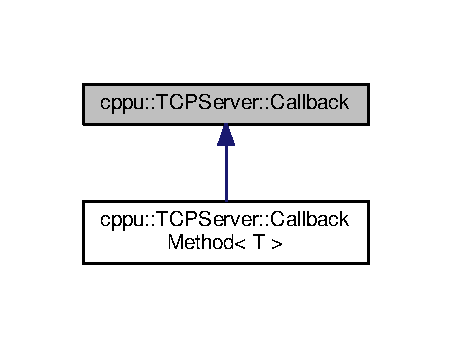
\includegraphics[width=217pt]{structcppu_1_1TCPServer_1_1Callback__inherit__graph}
\end{center}
\end{figure}
\subsection*{Public Member Functions}
\begin{DoxyCompactItemize}
\item 
virtual bool {\bfseries call} (\hyperlink{classcppu_1_1TCPConnection}{T\+C\+P\+Connection} \&cnx, const std\+::string \&request, std\+::string \&response)=0\hypertarget{structcppu_1_1TCPServer_1_1Callback_aabe4b0b30e14ddeb7c0c02aa3a335eba}{}\label{structcppu_1_1TCPServer_1_1Callback_aabe4b0b30e14ddeb7c0c02aa3a335eba}

\end{DoxyCompactItemize}


\subsection{Detailed Description}
\hyperlink{structcppu_1_1TCPServer_1_1Callback}{Callback} interface. 

The documentation for this struct was generated from the following file\+:\begin{DoxyCompactItemize}
\item 
tcpserver.\+h\end{DoxyCompactItemize}

\hypertarget{structcppu_1_1TCPServer_1_1CallbackMethod}{}\section{cppu\+:\+:T\+C\+P\+Server\+:\+:Callback\+Method$<$ T $>$ Struct Template Reference}
\label{structcppu_1_1TCPServer_1_1CallbackMethod}\index{cppu\+::\+T\+C\+P\+Server\+::\+Callback\+Method$<$ T $>$@{cppu\+::\+T\+C\+P\+Server\+::\+Callback\+Method$<$ T $>$}}


Inheritance diagram for cppu\+:\+:T\+C\+P\+Server\+:\+:Callback\+Method$<$ T $>$\+:\nopagebreak
\begin{figure}[H]
\begin{center}
\leavevmode
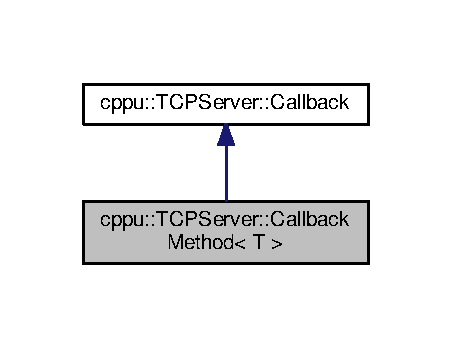
\includegraphics[width=217pt]{structcppu_1_1TCPServer_1_1CallbackMethod__inherit__graph}
\end{center}
\end{figure}


Collaboration diagram for cppu\+:\+:T\+C\+P\+Server\+:\+:Callback\+Method$<$ T $>$\+:\nopagebreak
\begin{figure}[H]
\begin{center}
\leavevmode
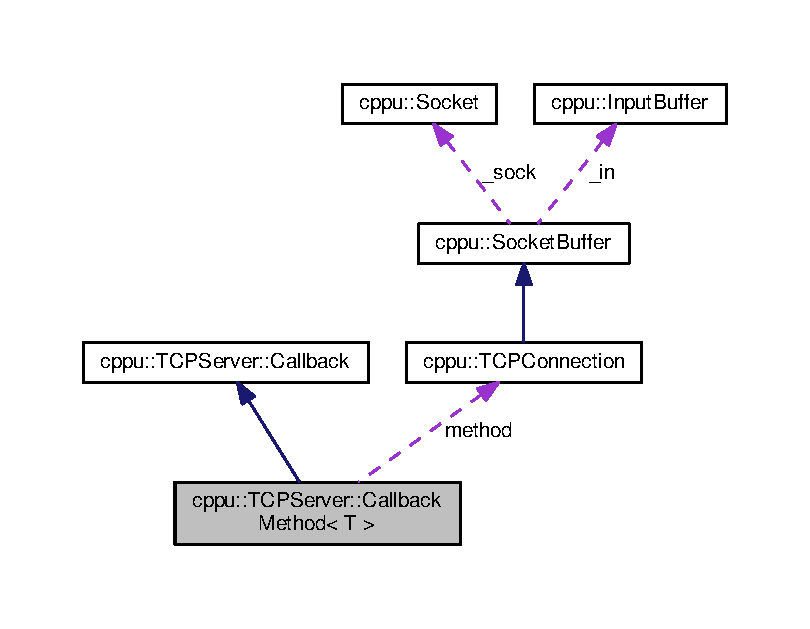
\includegraphics[width=350pt]{structcppu_1_1TCPServer_1_1CallbackMethod__coll__graph}
\end{center}
\end{figure}
\subsection*{Public Types}
\begin{DoxyCompactItemize}
\item 
typedef bool(T\+::$\ast$ {\bfseries Fun}) (\hyperlink{classcppu_1_1TCPConnection}{T\+C\+P\+Connection} \&, const std\+::string \&, std\+::string \&)\hypertarget{structcppu_1_1TCPServer_1_1CallbackMethod_a6f71d878bd072aadf40d96d1db18eecd}{}\label{structcppu_1_1TCPServer_1_1CallbackMethod_a6f71d878bd072aadf40d96d1db18eecd}

\end{DoxyCompactItemize}
\subsection*{Public Member Functions}
\begin{DoxyCompactItemize}
\item 
{\bfseries Callback\+Method} (T \&obj, Fun method)\hypertarget{structcppu_1_1TCPServer_1_1CallbackMethod_a0c6ceee6db8c67ef56fb26d1df52140f}{}\label{structcppu_1_1TCPServer_1_1CallbackMethod_a0c6ceee6db8c67ef56fb26d1df52140f}

\item 
virtual bool {\bfseries call} (\hyperlink{classcppu_1_1TCPConnection}{T\+C\+P\+Connection} \&cnx, const std\+::string \&req, std\+::string \&resp)\hypertarget{structcppu_1_1TCPServer_1_1CallbackMethod_a0c11039d0ed983c03a614d0764df3793}{}\label{structcppu_1_1TCPServer_1_1CallbackMethod_a0c11039d0ed983c03a614d0764df3793}

\end{DoxyCompactItemize}
\subsection*{Public Attributes}
\begin{DoxyCompactItemize}
\item 
T \& {\bfseries obj}\hypertarget{structcppu_1_1TCPServer_1_1CallbackMethod_ae480535d346efc119fb5c43880f349c8}{}\label{structcppu_1_1TCPServer_1_1CallbackMethod_ae480535d346efc119fb5c43880f349c8}

\item 
Fun {\bfseries method}\hypertarget{structcppu_1_1TCPServer_1_1CallbackMethod_aab858a039ddee71fb65a0e35c173f067}{}\label{structcppu_1_1TCPServer_1_1CallbackMethod_aab858a039ddee71fb65a0e35c173f067}

\end{DoxyCompactItemize}


The documentation for this struct was generated from the following file\+:\begin{DoxyCompactItemize}
\item 
tcpserver.\+h\end{DoxyCompactItemize}

\hypertarget{classFilm}{}\section{Film Class Reference}
\label{classFilm}\index{Film@{Film}}


{\ttfamily \#include $<$film.\+h$>$}



Inheritance diagram for Film\+:\nopagebreak
\begin{figure}[H]
\begin{center}
\leavevmode
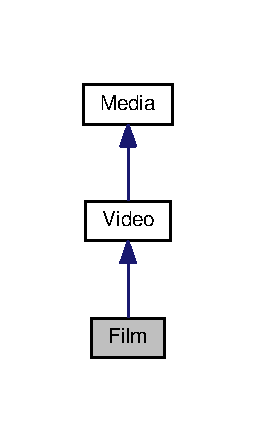
\includegraphics[width=123pt]{classFilm__inherit__graph}
\end{center}
\end{figure}


Collaboration diagram for Film\+:\nopagebreak
\begin{figure}[H]
\begin{center}
\leavevmode
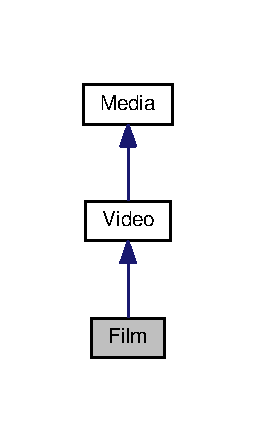
\includegraphics[width=123pt]{classFilm__coll__graph}
\end{center}
\end{figure}
\subsection*{Public Member Functions}
\begin{DoxyCompactItemize}
\item 
\hyperlink{classFilm_a8dab653f8a6c0635ca5ddbe0bbdd9a25}{$\sim$\+Film} ()
\item 
void \hyperlink{classFilm_a8024330b0d1317b147c053b47ce7bfac}{set\+Chapters} (const unsigned int chapters\mbox{[}$\,$\mbox{]}, const int length)
\item 
int \hyperlink{classFilm_a72227530aae37b57e2919d22fa1343ae}{get\+Chapters} (unsigned int $\ast$destination) const 
\item 
int \hyperlink{classFilm_a47c2898e2406de665bd31e00def57bfd}{get\+Number\+Chapters} () const 
\item 
void \hyperlink{classFilm_a7aa3acfe061d3af924529d761c29b74a}{print\+Chapters} () const 
\item 
string \hyperlink{classFilm_ab88f7ac028cd45da81c96a50a2990fee}{to\+String} () const 
\item 
string \hyperlink{classFilm_a660073fcb8d0c655ef49bc6d2c9a9ca1}{serialize} () const 
\end{DoxyCompactItemize}
\subsection*{Additional Inherited Members}


\subsection{Detailed Description}
Represents a movie, with chapters. 

\subsection{Constructor \& Destructor Documentation}
\index{Film@{Film}!````~Film@{$\sim$\+Film}}
\index{````~Film@{$\sim$\+Film}!Film@{Film}}
\subsubsection[{\texorpdfstring{$\sim$\+Film()}{~Film()}}]{\setlength{\rightskip}{0pt plus 5cm}Film\+::$\sim$\+Film (
\begin{DoxyParamCaption}
{}
\end{DoxyParamCaption}
)}\hypertarget{classFilm_a8dab653f8a6c0635ca5ddbe0bbdd9a25}{}\label{classFilm_a8dab653f8a6c0635ca5ddbe0bbdd9a25}
Destroys the object and its members. 

\subsection{Member Function Documentation}
\index{Film@{Film}!get\+Chapters@{get\+Chapters}}
\index{get\+Chapters@{get\+Chapters}!Film@{Film}}
\subsubsection[{\texorpdfstring{get\+Chapters(unsigned int $\ast$destination) const }{getChapters(unsigned int *destination) const }}]{\setlength{\rightskip}{0pt plus 5cm}int Film\+::get\+Chapters (
\begin{DoxyParamCaption}
\item[{unsigned int $\ast$}]{destination}
\end{DoxyParamCaption}
) const}\hypertarget{classFilm_a72227530aae37b57e2919d22fa1343ae}{}\label{classFilm_a72227530aae37b57e2919d22fa1343ae}
Returns the number of chapters and the array of chapters 
\begin{DoxyParams}{Parameters}
{\em destination} & a pointer to the destination array \\
\hline
\end{DoxyParams}
\begin{DoxyReturn}{Returns}
the number of chapters 
\end{DoxyReturn}
\index{Film@{Film}!get\+Number\+Chapters@{get\+Number\+Chapters}}
\index{get\+Number\+Chapters@{get\+Number\+Chapters}!Film@{Film}}
\subsubsection[{\texorpdfstring{get\+Number\+Chapters() const }{getNumberChapters() const }}]{\setlength{\rightskip}{0pt plus 5cm}int Film\+::get\+Number\+Chapters (
\begin{DoxyParamCaption}
{}
\end{DoxyParamCaption}
) const}\hypertarget{classFilm_a47c2898e2406de665bd31e00def57bfd}{}\label{classFilm_a47c2898e2406de665bd31e00def57bfd}
Returns the number of chapters \index{Film@{Film}!print\+Chapters@{print\+Chapters}}
\index{print\+Chapters@{print\+Chapters}!Film@{Film}}
\subsubsection[{\texorpdfstring{print\+Chapters() const }{printChapters() const }}]{\setlength{\rightskip}{0pt plus 5cm}void Film\+::print\+Chapters (
\begin{DoxyParamCaption}
{}
\end{DoxyParamCaption}
) const}\hypertarget{classFilm_a7aa3acfe061d3af924529d761c29b74a}{}\label{classFilm_a7aa3acfe061d3af924529d761c29b74a}
Prints each chapter and its length. \index{Film@{Film}!serialize@{serialize}}
\index{serialize@{serialize}!Film@{Film}}
\subsubsection[{\texorpdfstring{serialize() const }{serialize() const }}]{\setlength{\rightskip}{0pt plus 5cm}string Film\+::serialize (
\begin{DoxyParamCaption}
{}
\end{DoxyParamCaption}
) const\hspace{0.3cm}{\ttfamily [virtual]}}\hypertarget{classFilm_a660073fcb8d0c655ef49bc6d2c9a9ca1}{}\label{classFilm_a660073fcb8d0c655ef49bc6d2c9a9ca1}
Serializes the object. \begin{DoxyReturn}{Returns}
a string representing the object.
\end{DoxyReturn}
Format\+: \char`\"{}\+Film,\mbox{[}name\mbox{]},\mbox{[}path\mbox{]},\mbox{[}length\mbox{]},\mbox{[}n\mbox{]},\mbox{[}durations\mbox{]}\char`\"{}

where {\itshape n} is the number of chapters and {\itshape durations} is the list of the durations of each chapter, separated by the space character. e.\+g.\+: \char`\"{}\+Film,dog,$\sim$/\+Videos/dog.\+mkv,345,3,2 43 54\char`\"{} 

Implements \hyperlink{classMedia_ae588d20c062218e43b084da08f2dc5c6}{Media}.

\index{Film@{Film}!set\+Chapters@{set\+Chapters}}
\index{set\+Chapters@{set\+Chapters}!Film@{Film}}
\subsubsection[{\texorpdfstring{set\+Chapters(const unsigned int chapters[], const int length)}{setChapters(const unsigned int chapters[], const int length)}}]{\setlength{\rightskip}{0pt plus 5cm}void Film\+::set\+Chapters (
\begin{DoxyParamCaption}
\item[{const unsigned int}]{chapters\mbox{[}$\,$\mbox{]}, }
\item[{const int}]{length}
\end{DoxyParamCaption}
)}\hypertarget{classFilm_a8024330b0d1317b147c053b47ce7bfac}{}\label{classFilm_a8024330b0d1317b147c053b47ce7bfac}
Sets the length and number of chapters. 
\begin{DoxyParams}{Parameters}
{\em chapters} & the length of each chapter in seconds \\
\hline
{\em length} & the number of chapters \\
\hline
\end{DoxyParams}
\index{Film@{Film}!to\+String@{to\+String}}
\index{to\+String@{to\+String}!Film@{Film}}
\subsubsection[{\texorpdfstring{to\+String() const }{toString() const }}]{\setlength{\rightskip}{0pt plus 5cm}string Film\+::to\+String (
\begin{DoxyParamCaption}
{}
\end{DoxyParamCaption}
) const\hspace{0.3cm}{\ttfamily [virtual]}}\hypertarget{classFilm_ab88f7ac028cd45da81c96a50a2990fee}{}\label{classFilm_ab88f7ac028cd45da81c96a50a2990fee}
Prints a representation of the film in the standard output. 

Implements \hyperlink{classMedia_a95c1c019e23c2e365af1e5093d5232ac}{Media}.



The documentation for this class was generated from the following files\+:\begin{DoxyCompactItemize}
\item 
film.\+h\item 
film.\+cpp\end{DoxyCompactItemize}

\hypertarget{structcppu_1_1InputBuffer}{}\section{cppu\+:\+:Input\+Buffer Struct Reference}
\label{structcppu_1_1InputBuffer}\index{cppu\+::\+Input\+Buffer@{cppu\+::\+Input\+Buffer}}
\subsection*{Public Member Functions}
\begin{DoxyCompactItemize}
\item 
{\bfseries Input\+Buffer} (size\+\_\+t size)\hypertarget{structcppu_1_1InputBuffer_ac50e17e3cfb76a2983e5e3d4558b8144}{}\label{structcppu_1_1InputBuffer_ac50e17e3cfb76a2983e5e3d4558b8144}

\end{DoxyCompactItemize}
\subsection*{Public Attributes}
\begin{DoxyCompactItemize}
\item 
char $\ast$ {\bfseries buffer}\hypertarget{structcppu_1_1InputBuffer_a85138068e2e10731e46784b1552bc354}{}\label{structcppu_1_1InputBuffer_a85138068e2e10731e46784b1552bc354}

\item 
char $\ast$ {\bfseries begin}\hypertarget{structcppu_1_1InputBuffer_adbd6fb30fe51a192c9bbba6333016f31}{}\label{structcppu_1_1InputBuffer_adbd6fb30fe51a192c9bbba6333016f31}

\item 
char $\ast$ {\bfseries end}\hypertarget{structcppu_1_1InputBuffer_ac9fb4f51a6db191e71976fcda20237c0}{}\label{structcppu_1_1InputBuffer_ac9fb4f51a6db191e71976fcda20237c0}

\item 
ssize\+\_\+t {\bfseries remaining}\hypertarget{structcppu_1_1InputBuffer_a646b547733665524fa8b5de6b093ab11}{}\label{structcppu_1_1InputBuffer_a646b547733665524fa8b5de6b093ab11}

\end{DoxyCompactItemize}


The documentation for this struct was generated from the following file\+:\begin{DoxyCompactItemize}
\item 
cppsocket.\+cpp\end{DoxyCompactItemize}

\hypertarget{classMedia}{}\section{Media Class Reference}
\label{classMedia}\index{Media@{Media}}


{\ttfamily \#include $<$media.\+h$>$}



Inheritance diagram for Media\+:\nopagebreak
\begin{figure}[H]
\begin{center}
\leavevmode
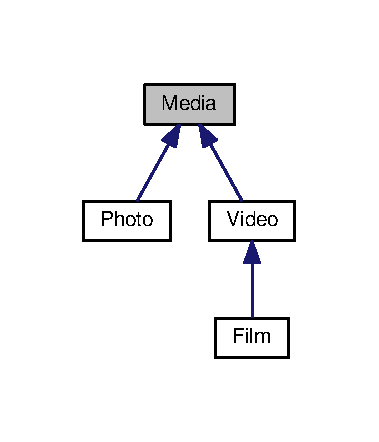
\includegraphics[width=182pt]{classMedia__inherit__graph}
\end{center}
\end{figure}
\subsection*{Public Member Functions}
\begin{DoxyCompactItemize}
\item 
\hyperlink{classMedia_a6e2ee1b8da6d724fb40a00ff4101d2df}{Media} ()
\item 
\hyperlink{classMedia_a0fcf9ae69f2d91790f3a1092dd867b91}{Media} (const string name, const string path)
\item 
void \hyperlink{classMedia_a51029a762fb97348c2accde515d10ff2}{set\+Name} (const string name)
\item 
string \hyperlink{classMedia_a6593900eea85ce823c5acad032339a1e}{get\+Name} () const 
\item 
void \hyperlink{classMedia_a309c0af39281e4621c5d32872008a2d7}{set\+Path} (const string path)
\item 
string \hyperlink{classMedia_ad2cbd7dec789109234a5db001a75153e}{get\+Path} () const 
\item 
void \hyperlink{classMedia_a62c3a585e2d7f5d0b8bb9617d8b4c3f5}{print} (ostream \&s) const 
\item 
virtual void \hyperlink{classMedia_aabbaa8413a9eeaccc649f9c3068ddbc6}{play} () const =0
\item 
virtual string \hyperlink{classMedia_a95c1c019e23c2e365af1e5093d5232ac}{to\+String} () const =0
\item 
virtual string \hyperlink{classMedia_ae588d20c062218e43b084da08f2dc5c6}{serialize} () const =0
\end{DoxyCompactItemize}
\subsection*{Protected Attributes}
\begin{DoxyCompactItemize}
\item 
string \hyperlink{classMedia_a853f210993023f79bf9606a9f86f9de3}{m\+\_\+name}
\item 
string \hyperlink{classMedia_abc2766c1b082546de88bff34e60f5809}{m\+\_\+path}
\end{DoxyCompactItemize}


\subsection{Detailed Description}
Class modeling multimedia objects 

\subsection{Constructor \& Destructor Documentation}
\index{Media@{Media}!Media@{Media}}
\index{Media@{Media}!Media@{Media}}
\subsubsection[{\texorpdfstring{Media()}{Media()}}]{\setlength{\rightskip}{0pt plus 5cm}Media\+::\+Media (
\begin{DoxyParamCaption}
{}
\end{DoxyParamCaption}
)}\hypertarget{classMedia_a6e2ee1b8da6d724fb40a00ff4101d2df}{}\label{classMedia_a6e2ee1b8da6d724fb40a00ff4101d2df}
Default constructor \index{Media@{Media}!Media@{Media}}
\index{Media@{Media}!Media@{Media}}
\subsubsection[{\texorpdfstring{Media(const string name, const string path)}{Media(const string name, const string path)}}]{\setlength{\rightskip}{0pt plus 5cm}Media\+::\+Media (
\begin{DoxyParamCaption}
\item[{const string}]{name, }
\item[{const string}]{path}
\end{DoxyParamCaption}
)}\hypertarget{classMedia_a0fcf9ae69f2d91790f3a1092dd867b91}{}\label{classMedia_a0fcf9ae69f2d91790f3a1092dd867b91}
Creates a media object with a name and a path to the file 
\begin{DoxyParams}{Parameters}
{\em name} & the name of the media \\
\hline
{\em path} & the path to the file, relative or absolute. \\
\hline
\end{DoxyParams}


\subsection{Member Function Documentation}
\index{Media@{Media}!get\+Name@{get\+Name}}
\index{get\+Name@{get\+Name}!Media@{Media}}
\subsubsection[{\texorpdfstring{get\+Name() const }{getName() const }}]{\setlength{\rightskip}{0pt plus 5cm}string Media\+::get\+Name (
\begin{DoxyParamCaption}
{}
\end{DoxyParamCaption}
) const}\hypertarget{classMedia_a6593900eea85ce823c5acad032339a1e}{}\label{classMedia_a6593900eea85ce823c5acad032339a1e}
Returns the name of the media \index{Media@{Media}!get\+Path@{get\+Path}}
\index{get\+Path@{get\+Path}!Media@{Media}}
\subsubsection[{\texorpdfstring{get\+Path() const }{getPath() const }}]{\setlength{\rightskip}{0pt plus 5cm}string Media\+::get\+Path (
\begin{DoxyParamCaption}
{}
\end{DoxyParamCaption}
) const}\hypertarget{classMedia_ad2cbd7dec789109234a5db001a75153e}{}\label{classMedia_ad2cbd7dec789109234a5db001a75153e}
Returns the path to the file represented by the object. \index{Media@{Media}!play@{play}}
\index{play@{play}!Media@{Media}}
\subsubsection[{\texorpdfstring{play() const =0}{play() const =0}}]{\setlength{\rightskip}{0pt plus 5cm}virtual void Media\+::play (
\begin{DoxyParamCaption}
{}
\end{DoxyParamCaption}
) const\hspace{0.3cm}{\ttfamily [pure virtual]}}\hypertarget{classMedia_aabbaa8413a9eeaccc649f9c3068ddbc6}{}\label{classMedia_aabbaa8413a9eeaccc649f9c3068ddbc6}
Play the media 

Implemented in \hyperlink{classVideo_acb8fdb5186d3b35672b9218375cf4f0b}{Video}, and \hyperlink{classPhoto_a34ef1c73e123d2951e8a08b3b1697c05}{Photo}.

\index{Media@{Media}!print@{print}}
\index{print@{print}!Media@{Media}}
\subsubsection[{\texorpdfstring{print(ostream \&s) const }{print(ostream &s) const }}]{\setlength{\rightskip}{0pt plus 5cm}void Media\+::print (
\begin{DoxyParamCaption}
\item[{ostream \&}]{s}
\end{DoxyParamCaption}
) const}\hypertarget{classMedia_a62c3a585e2d7f5d0b8bb9617d8b4c3f5}{}\label{classMedia_a62c3a585e2d7f5d0b8bb9617d8b4c3f5}
Prints the representation of the object. 
\begin{DoxyParams}{Parameters}
{\em s} & the outputstream that will print the representation \\
\hline
\end{DoxyParams}
\index{Media@{Media}!serialize@{serialize}}
\index{serialize@{serialize}!Media@{Media}}
\subsubsection[{\texorpdfstring{serialize() const =0}{serialize() const =0}}]{\setlength{\rightskip}{0pt plus 5cm}virtual string Media\+::serialize (
\begin{DoxyParamCaption}
{}
\end{DoxyParamCaption}
) const\hspace{0.3cm}{\ttfamily [pure virtual]}}\hypertarget{classMedia_ae588d20c062218e43b084da08f2dc5c6}{}\label{classMedia_ae588d20c062218e43b084da08f2dc5c6}
Returns a serialized representation of the media 

Implemented in \hyperlink{classFilm_a660073fcb8d0c655ef49bc6d2c9a9ca1}{Film}, \hyperlink{classVideo_a9360aa8a32752c7c732d993f2cf85144}{Video}, and \hyperlink{classPhoto_a6224b545b8795271c8225f6cccd80559}{Photo}.

\index{Media@{Media}!set\+Name@{set\+Name}}
\index{set\+Name@{set\+Name}!Media@{Media}}
\subsubsection[{\texorpdfstring{set\+Name(const string name)}{setName(const string name)}}]{\setlength{\rightskip}{0pt plus 5cm}void Media\+::set\+Name (
\begin{DoxyParamCaption}
\item[{const string}]{name}
\end{DoxyParamCaption}
)}\hypertarget{classMedia_a51029a762fb97348c2accde515d10ff2}{}\label{classMedia_a51029a762fb97348c2accde515d10ff2}
Sets the name of the media \index{Media@{Media}!set\+Path@{set\+Path}}
\index{set\+Path@{set\+Path}!Media@{Media}}
\subsubsection[{\texorpdfstring{set\+Path(const string path)}{setPath(const string path)}}]{\setlength{\rightskip}{0pt plus 5cm}void Media\+::set\+Path (
\begin{DoxyParamCaption}
\item[{const string}]{path}
\end{DoxyParamCaption}
)}\hypertarget{classMedia_a309c0af39281e4621c5d32872008a2d7}{}\label{classMedia_a309c0af39281e4621c5d32872008a2d7}
Sets the path to the file represented by the object. \index{Media@{Media}!to\+String@{to\+String}}
\index{to\+String@{to\+String}!Media@{Media}}
\subsubsection[{\texorpdfstring{to\+String() const =0}{toString() const =0}}]{\setlength{\rightskip}{0pt plus 5cm}virtual string Media\+::to\+String (
\begin{DoxyParamCaption}
{}
\end{DoxyParamCaption}
) const\hspace{0.3cm}{\ttfamily [pure virtual]}}\hypertarget{classMedia_a95c1c019e23c2e365af1e5093d5232ac}{}\label{classMedia_a95c1c019e23c2e365af1e5093d5232ac}
Returns a \char`\"{}pretty\char`\"{} representation of the media 

Implemented in \hyperlink{classFilm_ab88f7ac028cd45da81c96a50a2990fee}{Film}, \hyperlink{classVideo_ad947c70ddc192dcb8e511fda6a616a4f}{Video}, and \hyperlink{classPhoto_a72a86fd925fedd420e4367a529ed72cb}{Photo}.



\subsection{Member Data Documentation}
\index{Media@{Media}!m\+\_\+name@{m\+\_\+name}}
\index{m\+\_\+name@{m\+\_\+name}!Media@{Media}}
\subsubsection[{\texorpdfstring{m\+\_\+name}{m_name}}]{\setlength{\rightskip}{0pt plus 5cm}string Media\+::m\+\_\+name\hspace{0.3cm}{\ttfamily [protected]}}\hypertarget{classMedia_a853f210993023f79bf9606a9f86f9de3}{}\label{classMedia_a853f210993023f79bf9606a9f86f9de3}
Name of the media \index{Media@{Media}!m\+\_\+path@{m\+\_\+path}}
\index{m\+\_\+path@{m\+\_\+path}!Media@{Media}}
\subsubsection[{\texorpdfstring{m\+\_\+path}{m_path}}]{\setlength{\rightskip}{0pt plus 5cm}string Media\+::m\+\_\+path\hspace{0.3cm}{\ttfamily [protected]}}\hypertarget{classMedia_abc2766c1b082546de88bff34e60f5809}{}\label{classMedia_abc2766c1b082546de88bff34e60f5809}
Absolute or relative path 

The documentation for this class was generated from the following files\+:\begin{DoxyCompactItemize}
\item 
media.\+h\item 
media.\+cpp\end{DoxyCompactItemize}

\hypertarget{classMediaGroup}{}\section{Media\+Group Class Reference}
\label{classMediaGroup}\index{Media\+Group@{Media\+Group}}


{\ttfamily \#include $<$media\+Group.\+h$>$}



Inheritance diagram for Media\+Group\+:\nopagebreak
\begin{figure}[H]
\begin{center}
\leavevmode
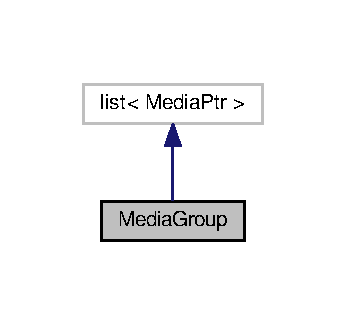
\includegraphics[width=166pt]{classMediaGroup__inherit__graph}
\end{center}
\end{figure}


Collaboration diagram for Media\+Group\+:\nopagebreak
\begin{figure}[H]
\begin{center}
\leavevmode
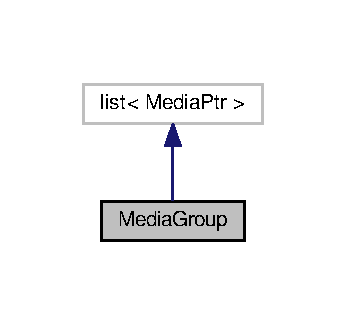
\includegraphics[width=166pt]{classMediaGroup__coll__graph}
\end{center}
\end{figure}
\subsection*{Public Member Functions}
\begin{DoxyCompactItemize}
\item 
\hyperlink{classMediaGroup_a64ae2f82091aab40c2c79c2679617b4d}{Media\+Group} ()
\item 
\hyperlink{classMediaGroup_a3c460f28adabb7b2525d7cb1f4f9e943}{Media\+Group} (string name)
\item 
void \hyperlink{classMediaGroup_ae1f711caf37c290bdd39f11412492fb2}{set\+Name} (string name)
\item 
string \hyperlink{classMediaGroup_af01d959a735d6ff95ccc7150dd87fee9}{get\+Name} ()
\item 
void \hyperlink{classMediaGroup_a2a0898010ea86c74133226295c95b0d3}{print\+All} ()
\item 
string \hyperlink{classMediaGroup_a24920081fe518357f1cb52fbd8c1bf17}{to\+String} ()
\end{DoxyCompactItemize}


\subsection{Detailed Description}
List of different medias 

\subsection{Constructor \& Destructor Documentation}
\index{Media\+Group@{Media\+Group}!Media\+Group@{Media\+Group}}
\index{Media\+Group@{Media\+Group}!Media\+Group@{Media\+Group}}
\subsubsection[{\texorpdfstring{Media\+Group()}{MediaGroup()}}]{\setlength{\rightskip}{0pt plus 5cm}Media\+Group\+::\+Media\+Group (
\begin{DoxyParamCaption}
{}
\end{DoxyParamCaption}
)}\hypertarget{classMediaGroup_a64ae2f82091aab40c2c79c2679617b4d}{}\label{classMediaGroup_a64ae2f82091aab40c2c79c2679617b4d}
Default constructor \index{Media\+Group@{Media\+Group}!Media\+Group@{Media\+Group}}
\index{Media\+Group@{Media\+Group}!Media\+Group@{Media\+Group}}
\subsubsection[{\texorpdfstring{Media\+Group(string name)}{MediaGroup(string name)}}]{\setlength{\rightskip}{0pt plus 5cm}Media\+Group\+::\+Media\+Group (
\begin{DoxyParamCaption}
\item[{string}]{name}
\end{DoxyParamCaption}
)}\hypertarget{classMediaGroup_a3c460f28adabb7b2525d7cb1f4f9e943}{}\label{classMediaGroup_a3c460f28adabb7b2525d7cb1f4f9e943}
Creates a new group and sets the name. 

\subsection{Member Function Documentation}
\index{Media\+Group@{Media\+Group}!get\+Name@{get\+Name}}
\index{get\+Name@{get\+Name}!Media\+Group@{Media\+Group}}
\subsubsection[{\texorpdfstring{get\+Name()}{getName()}}]{\setlength{\rightskip}{0pt plus 5cm}string Media\+Group\+::get\+Name (
\begin{DoxyParamCaption}
{}
\end{DoxyParamCaption}
)}\hypertarget{classMediaGroup_af01d959a735d6ff95ccc7150dd87fee9}{}\label{classMediaGroup_af01d959a735d6ff95ccc7150dd87fee9}
Returns the name of the group \index{Media\+Group@{Media\+Group}!print\+All@{print\+All}}
\index{print\+All@{print\+All}!Media\+Group@{Media\+Group}}
\subsubsection[{\texorpdfstring{print\+All()}{printAll()}}]{\setlength{\rightskip}{0pt plus 5cm}void Media\+Group\+::print\+All (
\begin{DoxyParamCaption}
{}
\end{DoxyParamCaption}
)}\hypertarget{classMediaGroup_a2a0898010ea86c74133226295c95b0d3}{}\label{classMediaGroup_a2a0898010ea86c74133226295c95b0d3}
Print all media stored in the group to the standard output \index{Media\+Group@{Media\+Group}!set\+Name@{set\+Name}}
\index{set\+Name@{set\+Name}!Media\+Group@{Media\+Group}}
\subsubsection[{\texorpdfstring{set\+Name(string name)}{setName(string name)}}]{\setlength{\rightskip}{0pt plus 5cm}void Media\+Group\+::set\+Name (
\begin{DoxyParamCaption}
\item[{string}]{name}
\end{DoxyParamCaption}
)}\hypertarget{classMediaGroup_ae1f711caf37c290bdd39f11412492fb2}{}\label{classMediaGroup_ae1f711caf37c290bdd39f11412492fb2}
Sets the name of the group \index{Media\+Group@{Media\+Group}!to\+String@{to\+String}}
\index{to\+String@{to\+String}!Media\+Group@{Media\+Group}}
\subsubsection[{\texorpdfstring{to\+String()}{toString()}}]{\setlength{\rightskip}{0pt plus 5cm}string Media\+Group\+::to\+String (
\begin{DoxyParamCaption}
{}
\end{DoxyParamCaption}
)}\hypertarget{classMediaGroup_a24920081fe518357f1cb52fbd8c1bf17}{}\label{classMediaGroup_a24920081fe518357f1cb52fbd8c1bf17}
Returns a human-\/readable representation of the group 

The documentation for this class was generated from the following files\+:\begin{DoxyCompactItemize}
\item 
media\+Group.\+h\item 
media\+Group.\+cpp\end{DoxyCompactItemize}

\hypertarget{classMediaStorage}{}\section{Media\+Storage Class Reference}
\label{classMediaStorage}\index{Media\+Storage@{Media\+Storage}}
\subsection*{Static Public Member Functions}
\begin{DoxyCompactItemize}
\item 
static Media\+Ptr \hyperlink{classMediaStorage_afd1c58d3d41cf932b0b091d346726996}{find\+Media} (string srch)
\item 
static Media\+Grp\+Ptr \hyperlink{classMediaStorage_afbc1491a61445a0fa70c69e4c78be356}{find\+Media\+Grp} (string srch)
\item 
static void \hyperlink{classMediaStorage_a53a717cd521376ef1d38bba485fff218}{play\+Media} (const string name)
\item 
static void \hyperlink{classMediaStorage_ac9f6b5047a11a5123c09885155cff2e0}{print\+Media} (const string name)
\item 
static void \hyperlink{classMediaStorage_abf9dcfa0c6647f32816f3cab13eb325b}{print\+Group} (const string name)
\item 
static void \hyperlink{classMediaStorage_a38497104de3ebadf0968e55e29b7e7ef}{print\+All\+Media} ()
\item 
static void \hyperlink{classMediaStorage_aad266fb25546eee62037193b533ac10a}{print\+All\+Grp} ()
\item 
static shared\+\_\+ptr$<$ \hyperlink{classPhoto}{Photo} $>$ \hyperlink{classMediaStorage_a22db05b2288f4ea728506fa632205335}{new\+Photo} (string name, string path)
\item 
static shared\+\_\+ptr$<$ \hyperlink{classVideo}{Video} $>$ \hyperlink{classMediaStorage_aec1d47d5d30f17bdb6ae443e464c4bd4}{new\+Video} (string name, string path)
\item 
static shared\+\_\+ptr$<$ \hyperlink{classFilm}{Film} $>$ \hyperlink{classMediaStorage_a55db96df35aae1348581b6fbc27a34bc}{new\+Film} (string name, string path)
\item 
static Media\+Grp\+Ptr \hyperlink{classMediaStorage_a0762b1452654e6d47fa93d7ad5001520}{new\+Media\+Grp} (string name)
\item 
static void \hyperlink{classMediaStorage_ae0c7f77a76c3496bfea91145ebd4acc5}{remove\+Media} (string name)
\item 
static void \hyperlink{classMediaStorage_a295d0fe139b82b0fbb351e17ee7759dd}{remove\+Group} (string name)
\item 
static string \hyperlink{classMediaStorage_a93e1a78d314ecb11e1024c322fa670f3}{handle\+Request} (string request)
\item 
static Media\+Ptr \hyperlink{classMediaStorage_a9a5a91b418dd9da61ca394f789c557fb}{from\+String} (string serialized)
\end{DoxyCompactItemize}


\subsection{Member Function Documentation}
\index{Media\+Storage@{Media\+Storage}!find\+Media@{find\+Media}}
\index{find\+Media@{find\+Media}!Media\+Storage@{Media\+Storage}}
\subsubsection[{\texorpdfstring{find\+Media(string srch)}{findMedia(string srch)}}]{\setlength{\rightskip}{0pt plus 5cm}Media\+Ptr Media\+Storage\+::find\+Media (
\begin{DoxyParamCaption}
\item[{string}]{srch}
\end{DoxyParamCaption}
)\hspace{0.3cm}{\ttfamily [static]}}\hypertarget{classMediaStorage_afd1c58d3d41cf932b0b091d346726996}{}\label{classMediaStorage_afd1c58d3d41cf932b0b091d346726996}
Find a media by name 
\begin{DoxyParams}{Parameters}
{\em srch} & The name of the searched media \\
\hline
\end{DoxyParams}
\begin{DoxyReturn}{Returns}
a pointer to the object, or {\ttfamily nullptr} if nothing is found. 
\end{DoxyReturn}
\index{Media\+Storage@{Media\+Storage}!find\+Media\+Grp@{find\+Media\+Grp}}
\index{find\+Media\+Grp@{find\+Media\+Grp}!Media\+Storage@{Media\+Storage}}
\subsubsection[{\texorpdfstring{find\+Media\+Grp(string srch)}{findMediaGrp(string srch)}}]{\setlength{\rightskip}{0pt plus 5cm}Media\+Grp\+Ptr Media\+Storage\+::find\+Media\+Grp (
\begin{DoxyParamCaption}
\item[{string}]{srch}
\end{DoxyParamCaption}
)\hspace{0.3cm}{\ttfamily [static]}}\hypertarget{classMediaStorage_afbc1491a61445a0fa70c69e4c78be356}{}\label{classMediaStorage_afbc1491a61445a0fa70c69e4c78be356}
Find a group by name 
\begin{DoxyParams}{Parameters}
{\em srch} & The name of the searched group \\
\hline
\end{DoxyParams}
\begin{DoxyReturn}{Returns}
a pointer to the group, or {\ttfamily nullptr} if nothing is found. 
\end{DoxyReturn}
\index{Media\+Storage@{Media\+Storage}!from\+String@{from\+String}}
\index{from\+String@{from\+String}!Media\+Storage@{Media\+Storage}}
\subsubsection[{\texorpdfstring{from\+String(string serialized)}{fromString(string serialized)}}]{\setlength{\rightskip}{0pt plus 5cm}Media\+Ptr Media\+Storage\+::from\+String (
\begin{DoxyParamCaption}
\item[{string}]{serialized}
\end{DoxyParamCaption}
)\hspace{0.3cm}{\ttfamily [static]}}\hypertarget{classMediaStorage_a9a5a91b418dd9da61ca394f789c557fb}{}\label{classMediaStorage_a9a5a91b418dd9da61ca394f789c557fb}
Create a new object from a serialized representation \index{Media\+Storage@{Media\+Storage}!handle\+Request@{handle\+Request}}
\index{handle\+Request@{handle\+Request}!Media\+Storage@{Media\+Storage}}
\subsubsection[{\texorpdfstring{handle\+Request(string request)}{handleRequest(string request)}}]{\setlength{\rightskip}{0pt plus 5cm}string Media\+Storage\+::handle\+Request (
\begin{DoxyParamCaption}
\item[{string}]{request}
\end{DoxyParamCaption}
)\hspace{0.3cm}{\ttfamily [static]}}\hypertarget{classMediaStorage_a93e1a78d314ecb11e1024c322fa670f3}{}\label{classMediaStorage_a93e1a78d314ecb11e1024c322fa670f3}
Process a request from a client 
\begin{DoxyParams}{Parameters}
{\em request} & A well formatted request.\\
\hline
\end{DoxyParams}
e.\+g.\+: \char`\"{}print \mbox{[}name of media\mbox{]}\char`\"{} or \char`\"{}play \mbox{[}name of media\mbox{]}\char`\"{} \begin{DoxyReturn}{Returns}
the response 
\end{DoxyReturn}
\index{Media\+Storage@{Media\+Storage}!new\+Film@{new\+Film}}
\index{new\+Film@{new\+Film}!Media\+Storage@{Media\+Storage}}
\subsubsection[{\texorpdfstring{new\+Film(string name, string path)}{newFilm(string name, string path)}}]{\setlength{\rightskip}{0pt plus 5cm}shared\+\_\+ptr$<$ {\bf Film} $>$ Media\+Storage\+::new\+Film (
\begin{DoxyParamCaption}
\item[{string}]{name, }
\item[{string}]{path}
\end{DoxyParamCaption}
)\hspace{0.3cm}{\ttfamily [static]}}\hypertarget{classMediaStorage_a55db96df35aae1348581b6fbc27a34bc}{}\label{classMediaStorage_a55db96df35aae1348581b6fbc27a34bc}
Create a new film 
\begin{DoxyParams}{Parameters}
{\em name} & The name of the film \\
\hline
{\em path} & The location of the file \\
\hline
\end{DoxyParams}
\begin{DoxyReturn}{Returns}
a shared pointer to the object 
\end{DoxyReturn}

\begin{DoxyExceptions}{Exceptions}
{\em runtime\+\_\+error} & if there is already a media object with the same name. \\
\hline
\end{DoxyExceptions}
\index{Media\+Storage@{Media\+Storage}!new\+Media\+Grp@{new\+Media\+Grp}}
\index{new\+Media\+Grp@{new\+Media\+Grp}!Media\+Storage@{Media\+Storage}}
\subsubsection[{\texorpdfstring{new\+Media\+Grp(string name)}{newMediaGrp(string name)}}]{\setlength{\rightskip}{0pt plus 5cm}Media\+Grp\+Ptr Media\+Storage\+::new\+Media\+Grp (
\begin{DoxyParamCaption}
\item[{string}]{name}
\end{DoxyParamCaption}
)\hspace{0.3cm}{\ttfamily [static]}}\hypertarget{classMediaStorage_a0762b1452654e6d47fa93d7ad5001520}{}\label{classMediaStorage_a0762b1452654e6d47fa93d7ad5001520}
Create a new group of media 
\begin{DoxyParams}{Parameters}
{\em name} & The name of the group \\
\hline
\end{DoxyParams}
\begin{DoxyReturn}{Returns}
a shared pointer to the object 
\end{DoxyReturn}

\begin{DoxyExceptions}{Exceptions}
{\em runtime\+\_\+error} & if there is already a group with the same name. \\
\hline
\end{DoxyExceptions}
\index{Media\+Storage@{Media\+Storage}!new\+Photo@{new\+Photo}}
\index{new\+Photo@{new\+Photo}!Media\+Storage@{Media\+Storage}}
\subsubsection[{\texorpdfstring{new\+Photo(string name, string path)}{newPhoto(string name, string path)}}]{\setlength{\rightskip}{0pt plus 5cm}shared\+\_\+ptr$<$ {\bf Photo} $>$ Media\+Storage\+::new\+Photo (
\begin{DoxyParamCaption}
\item[{string}]{name, }
\item[{string}]{path}
\end{DoxyParamCaption}
)\hspace{0.3cm}{\ttfamily [static]}}\hypertarget{classMediaStorage_a22db05b2288f4ea728506fa632205335}{}\label{classMediaStorage_a22db05b2288f4ea728506fa632205335}
Create a new photo 
\begin{DoxyParams}{Parameters}
{\em name} & The name of the photo \\
\hline
{\em path} & The location of the file \\
\hline
\end{DoxyParams}
\begin{DoxyReturn}{Returns}
a shared pointer to the object 
\end{DoxyReturn}

\begin{DoxyExceptions}{Exceptions}
{\em runtime\+\_\+error} & if there is already a media object with the same name. \\
\hline
\end{DoxyExceptions}
\index{Media\+Storage@{Media\+Storage}!new\+Video@{new\+Video}}
\index{new\+Video@{new\+Video}!Media\+Storage@{Media\+Storage}}
\subsubsection[{\texorpdfstring{new\+Video(string name, string path)}{newVideo(string name, string path)}}]{\setlength{\rightskip}{0pt plus 5cm}shared\+\_\+ptr$<$ {\bf Video} $>$ Media\+Storage\+::new\+Video (
\begin{DoxyParamCaption}
\item[{string}]{name, }
\item[{string}]{path}
\end{DoxyParamCaption}
)\hspace{0.3cm}{\ttfamily [static]}}\hypertarget{classMediaStorage_aec1d47d5d30f17bdb6ae443e464c4bd4}{}\label{classMediaStorage_aec1d47d5d30f17bdb6ae443e464c4bd4}
Create a new video 
\begin{DoxyParams}{Parameters}
{\em name} & The name of the video \\
\hline
{\em path} & The location of the file \\
\hline
\end{DoxyParams}
\begin{DoxyReturn}{Returns}
a shared pointer to the object 
\end{DoxyReturn}

\begin{DoxyExceptions}{Exceptions}
{\em runtime\+\_\+error} & if there is already a media object with the same name. \\
\hline
\end{DoxyExceptions}
\index{Media\+Storage@{Media\+Storage}!play\+Media@{play\+Media}}
\index{play\+Media@{play\+Media}!Media\+Storage@{Media\+Storage}}
\subsubsection[{\texorpdfstring{play\+Media(const string name)}{playMedia(const string name)}}]{\setlength{\rightskip}{0pt plus 5cm}void Media\+Storage\+::play\+Media (
\begin{DoxyParamCaption}
\item[{const string}]{name}
\end{DoxyParamCaption}
)\hspace{0.3cm}{\ttfamily [static]}}\hypertarget{classMediaStorage_a53a717cd521376ef1d38bba485fff218}{}\label{classMediaStorage_a53a717cd521376ef1d38bba485fff218}
Play a media 
\begin{DoxyParams}{Parameters}
{\em name} & The name of the media \\
\hline
\end{DoxyParams}

\begin{DoxyExceptions}{Exceptions}
{\em runtime\+\_\+error} & if the media is not found \\
\hline
\end{DoxyExceptions}
\index{Media\+Storage@{Media\+Storage}!print\+All\+Grp@{print\+All\+Grp}}
\index{print\+All\+Grp@{print\+All\+Grp}!Media\+Storage@{Media\+Storage}}
\subsubsection[{\texorpdfstring{print\+All\+Grp()}{printAllGrp()}}]{\setlength{\rightskip}{0pt plus 5cm}void Media\+Storage\+::print\+All\+Grp (
\begin{DoxyParamCaption}
{}
\end{DoxyParamCaption}
)\hspace{0.3cm}{\ttfamily [static]}}\hypertarget{classMediaStorage_aad266fb25546eee62037193b533ac10a}{}\label{classMediaStorage_aad266fb25546eee62037193b533ac10a}
Prints a human-\/readable representation of all the stored groups \index{Media\+Storage@{Media\+Storage}!print\+All\+Media@{print\+All\+Media}}
\index{print\+All\+Media@{print\+All\+Media}!Media\+Storage@{Media\+Storage}}
\subsubsection[{\texorpdfstring{print\+All\+Media()}{printAllMedia()}}]{\setlength{\rightskip}{0pt plus 5cm}void Media\+Storage\+::print\+All\+Media (
\begin{DoxyParamCaption}
{}
\end{DoxyParamCaption}
)\hspace{0.3cm}{\ttfamily [static]}}\hypertarget{classMediaStorage_a38497104de3ebadf0968e55e29b7e7ef}{}\label{classMediaStorage_a38497104de3ebadf0968e55e29b7e7ef}
Prints a human-\/readable representation of all the stored media \index{Media\+Storage@{Media\+Storage}!print\+Group@{print\+Group}}
\index{print\+Group@{print\+Group}!Media\+Storage@{Media\+Storage}}
\subsubsection[{\texorpdfstring{print\+Group(const string name)}{printGroup(const string name)}}]{\setlength{\rightskip}{0pt plus 5cm}void Media\+Storage\+::print\+Group (
\begin{DoxyParamCaption}
\item[{const string}]{name}
\end{DoxyParamCaption}
)\hspace{0.3cm}{\ttfamily [static]}}\hypertarget{classMediaStorage_abf9dcfa0c6647f32816f3cab13eb325b}{}\label{classMediaStorage_abf9dcfa0c6647f32816f3cab13eb325b}
Prints a human-\/readable representation of the group in the standard output 
\begin{DoxyParams}{Parameters}
{\em name} & The name of the group \\
\hline
\end{DoxyParams}

\begin{DoxyExceptions}{Exceptions}
{\em runtime\+\_\+error} & if the group is not found \\
\hline
\end{DoxyExceptions}
\index{Media\+Storage@{Media\+Storage}!print\+Media@{print\+Media}}
\index{print\+Media@{print\+Media}!Media\+Storage@{Media\+Storage}}
\subsubsection[{\texorpdfstring{print\+Media(const string name)}{printMedia(const string name)}}]{\setlength{\rightskip}{0pt plus 5cm}void Media\+Storage\+::print\+Media (
\begin{DoxyParamCaption}
\item[{const string}]{name}
\end{DoxyParamCaption}
)\hspace{0.3cm}{\ttfamily [static]}}\hypertarget{classMediaStorage_ac9f6b5047a11a5123c09885155cff2e0}{}\label{classMediaStorage_ac9f6b5047a11a5123c09885155cff2e0}
Prints a human-\/readable representation of the media in the standard output 
\begin{DoxyParams}{Parameters}
{\em name} & The name of the media \\
\hline
\end{DoxyParams}

\begin{DoxyExceptions}{Exceptions}
{\em runtime\+\_\+error} & if the media is not found \\
\hline
\end{DoxyExceptions}
\index{Media\+Storage@{Media\+Storage}!remove\+Group@{remove\+Group}}
\index{remove\+Group@{remove\+Group}!Media\+Storage@{Media\+Storage}}
\subsubsection[{\texorpdfstring{remove\+Group(string name)}{removeGroup(string name)}}]{\setlength{\rightskip}{0pt plus 5cm}void Media\+Storage\+::remove\+Group (
\begin{DoxyParamCaption}
\item[{string}]{name}
\end{DoxyParamCaption}
)\hspace{0.3cm}{\ttfamily [static]}}\hypertarget{classMediaStorage_a295d0fe139b82b0fbb351e17ee7759dd}{}\label{classMediaStorage_a295d0fe139b82b0fbb351e17ee7759dd}
Remove a group object 
\begin{DoxyParams}{Parameters}
{\em name} & The name of the group \\
\hline
\end{DoxyParams}

\begin{DoxyExceptions}{Exceptions}
{\em runtime\+\_\+error} & if there is no stored group with this name \\
\hline
\end{DoxyExceptions}
\index{Media\+Storage@{Media\+Storage}!remove\+Media@{remove\+Media}}
\index{remove\+Media@{remove\+Media}!Media\+Storage@{Media\+Storage}}
\subsubsection[{\texorpdfstring{remove\+Media(string name)}{removeMedia(string name)}}]{\setlength{\rightskip}{0pt plus 5cm}void Media\+Storage\+::remove\+Media (
\begin{DoxyParamCaption}
\item[{string}]{name}
\end{DoxyParamCaption}
)\hspace{0.3cm}{\ttfamily [static]}}\hypertarget{classMediaStorage_ae0c7f77a76c3496bfea91145ebd4acc5}{}\label{classMediaStorage_ae0c7f77a76c3496bfea91145ebd4acc5}
Remove a media object 
\begin{DoxyParams}{Parameters}
{\em name} & The name of the media \\
\hline
\end{DoxyParams}

\begin{DoxyExceptions}{Exceptions}
{\em runtime\+\_\+error} & if there is no stored media with this name \\
\hline
\end{DoxyExceptions}


The documentation for this class was generated from the following files\+:\begin{DoxyCompactItemize}
\item 
media\+Storage.\+h\item 
media\+Storage.\+cpp\end{DoxyCompactItemize}

\hypertarget{classMyBase}{}\section{My\+Base Class Reference}
\label{classMyBase}\index{My\+Base@{My\+Base}}
\subsection*{Public Member Functions}
\begin{DoxyCompactItemize}
\item 
bool \hyperlink{classMyBase_a818864f09718a0aa6d65f5ac5733b689}{process\+Request} (\hyperlink{classcppu_1_1TCPConnection}{T\+C\+P\+Connection} \&cnx, const string \&request, string \&response)
\end{DoxyCompactItemize}


\subsection{Member Function Documentation}
\index{My\+Base@{My\+Base}!process\+Request@{process\+Request}}
\index{process\+Request@{process\+Request}!My\+Base@{My\+Base}}
\subsubsection[{\texorpdfstring{process\+Request(\+T\+C\+P\+Connection \&cnx, const string \&request, string \&response)}{processRequest(TCPConnection &cnx, const string &request, string &response)}}]{\setlength{\rightskip}{0pt plus 5cm}bool My\+Base\+::process\+Request (
\begin{DoxyParamCaption}
\item[{{\bf T\+C\+P\+Connection} \&}]{cnx, }
\item[{const string \&}]{request, }
\item[{string \&}]{response}
\end{DoxyParamCaption}
)\hspace{0.3cm}{\ttfamily [inline]}}\hypertarget{classMyBase_a818864f09718a0aa6d65f5ac5733b689}{}\label{classMyBase_a818864f09718a0aa6d65f5ac5733b689}
Method called for each request 
\begin{DoxyParams}{Parameters}
{\em cnx} & \\
\hline
{\em request} & the request sent by the client \\
\hline
{\em response} & the answer to send to the client \\
\hline
\end{DoxyParams}
\begin{DoxyReturn}{Returns}
true if everything went fine, or false if we want to end to end the connection. 
\end{DoxyReturn}


The documentation for this class was generated from the following file\+:\begin{DoxyCompactItemize}
\item 
main.\+cpp\end{DoxyCompactItemize}

\hypertarget{classPhoto}{}\section{Photo Class Reference}
\label{classPhoto}\index{Photo@{Photo}}


Inheritance diagram for Photo\+:\nopagebreak
\begin{figure}[H]
\begin{center}
\leavevmode
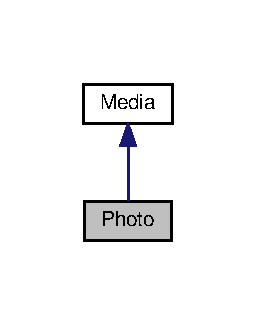
\includegraphics[width=123pt]{classPhoto__inherit__graph}
\end{center}
\end{figure}


Collaboration diagram for Photo\+:\nopagebreak
\begin{figure}[H]
\begin{center}
\leavevmode
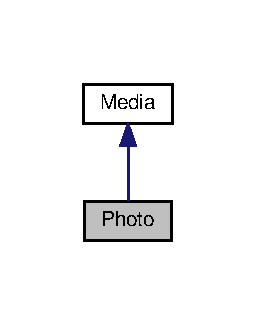
\includegraphics[width=123pt]{classPhoto__coll__graph}
\end{center}
\end{figure}
\subsection*{Public Member Functions}
\begin{DoxyCompactItemize}
\item 
void \hyperlink{classPhoto_a34ef1c73e123d2951e8a08b3b1697c05}{play} () const 
\item 
void {\bfseries set\+Latitude} (const float lat)\hypertarget{classPhoto_a49c4e44e93f85879e31c52178e324a7d}{}\label{classPhoto_a49c4e44e93f85879e31c52178e324a7d}

\item 
float {\bfseries get\+Latitude} () const \hypertarget{classPhoto_a26808b7206b3510e31f6dd38146e7710}{}\label{classPhoto_a26808b7206b3510e31f6dd38146e7710}

\item 
void {\bfseries set\+Longitude} (const float longi)\hypertarget{classPhoto_abd3795ba4724e9c881c0761fc8858ebd}{}\label{classPhoto_abd3795ba4724e9c881c0761fc8858ebd}

\item 
float {\bfseries get\+Longitude} () const \hypertarget{classPhoto_a02787b27b9d7c919e9ecfaa2e99a1862}{}\label{classPhoto_a02787b27b9d7c919e9ecfaa2e99a1862}

\item 
string \hyperlink{classPhoto_a72a86fd925fedd420e4367a529ed72cb}{to\+String} () const 
\item 
string \hyperlink{classPhoto_a6224b545b8795271c8225f6cccd80559}{serialize} () const 
\end{DoxyCompactItemize}
\subsection*{Additional Inherited Members}


\subsection{Member Function Documentation}
\index{Photo@{Photo}!play@{play}}
\index{play@{play}!Photo@{Photo}}
\subsubsection[{\texorpdfstring{play() const }{play() const }}]{\setlength{\rightskip}{0pt plus 5cm}void Photo\+::play (
\begin{DoxyParamCaption}
{}
\end{DoxyParamCaption}
) const\hspace{0.3cm}{\ttfamily [virtual]}}\hypertarget{classPhoto_a34ef1c73e123d2951e8a08b3b1697c05}{}\label{classPhoto_a34ef1c73e123d2951e8a08b3b1697c05}
Play the media 

Implements \hyperlink{classMedia_aabbaa8413a9eeaccc649f9c3068ddbc6}{Media}.

\index{Photo@{Photo}!serialize@{serialize}}
\index{serialize@{serialize}!Photo@{Photo}}
\subsubsection[{\texorpdfstring{serialize() const }{serialize() const }}]{\setlength{\rightskip}{0pt plus 5cm}string Photo\+::serialize (
\begin{DoxyParamCaption}
{}
\end{DoxyParamCaption}
) const\hspace{0.3cm}{\ttfamily [virtual]}}\hypertarget{classPhoto_a6224b545b8795271c8225f6cccd80559}{}\label{classPhoto_a6224b545b8795271c8225f6cccd80559}
Returns a serialized representation of the object \begin{DoxyReturn}{Returns}
the representation of the object in the format \char`\"{}\+Photo,\mbox{[}name\mbox{]},\mbox{[}path\mbox{]},\mbox{[}latitude\mbox{]},\mbox{[}longitude\mbox{]}\char`\"{}
\end{DoxyReturn}
e.\+g. \char`\"{}\+Photo,dog,$\sim$/\+Photos/dog.\+jpg,34.\+5,65.\+4\char`\"{} 

Implements \hyperlink{classMedia_ae588d20c062218e43b084da08f2dc5c6}{Media}.

\index{Photo@{Photo}!to\+String@{to\+String}}
\index{to\+String@{to\+String}!Photo@{Photo}}
\subsubsection[{\texorpdfstring{to\+String() const }{toString() const }}]{\setlength{\rightskip}{0pt plus 5cm}string Photo\+::to\+String (
\begin{DoxyParamCaption}
{}
\end{DoxyParamCaption}
) const\hspace{0.3cm}{\ttfamily [virtual]}}\hypertarget{classPhoto_a72a86fd925fedd420e4367a529ed72cb}{}\label{classPhoto_a72a86fd925fedd420e4367a529ed72cb}
Returns an human-\/readable representation of the object. 

Implements \hyperlink{classMedia_a95c1c019e23c2e365af1e5093d5232ac}{Media}.



The documentation for this class was generated from the following files\+:\begin{DoxyCompactItemize}
\item 
photo.\+h\item 
photo.\+cpp\end{DoxyCompactItemize}

\hypertarget{classcppu_1_1ServerSocket}{}\section{cppu\+:\+:Server\+Socket Class Reference}
\label{classcppu_1_1ServerSocket}\index{cppu\+::\+Server\+Socket@{cppu\+::\+Server\+Socket}}


T\+C\+P/\+IP server socket. This class implements a T\+C\+P/\+IP socket that waits for requests to come in over the network. A\+F\+\_\+\+I\+N\+ET connections following the I\+Pv4 Internet protocol are supported.  




{\ttfamily \#include $<$cppsocket.\+h$>$}

\subsection*{Public Member Functions}
\begin{DoxyCompactItemize}
\item 
\hyperlink{classcppu_1_1ServerSocket_a57138f5a7d2e8af35228c8985385c494}{Server\+Socket} ()\hypertarget{classcppu_1_1ServerSocket_a57138f5a7d2e8af35228c8985385c494}{}\label{classcppu_1_1ServerSocket_a57138f5a7d2e8af35228c8985385c494}

\begin{DoxyCompactList}\small\item\em Creates a new server socket. Creates a listening socket that waits for connection requests by T\+C\+P/\+IP clients. \end{DoxyCompactList}\item 
virtual \hyperlink{classcppu_1_1Socket}{Socket} $\ast$ \hyperlink{classcppu_1_1ServerSocket_af08ebcb886fc778d195fb622f7b96b8b}{accept} ()
\begin{DoxyCompactList}\small\item\em Accepts a new connection request and returns the corresponding socket. By default, this function blocks the caller until a connection is present. \end{DoxyCompactList}\item 
virtual int \hyperlink{classcppu_1_1ServerSocket_a255dfdccba51c7cdbcb6733c6c3f6ffa}{bind} (int port, int backlog=50)
\begin{DoxyCompactList}\small\item\em Assigns the socket to the local address. The socket must be bound before using it. \end{DoxyCompactList}\item 
virtual int \hyperlink{classcppu_1_1ServerSocket_ae7647cfb5beaf504a846f6ecfdd197c4}{close} ()\hypertarget{classcppu_1_1ServerSocket_ae7647cfb5beaf504a846f6ecfdd197c4}{}\label{classcppu_1_1ServerSocket_ae7647cfb5beaf504a846f6ecfdd197c4}

\begin{DoxyCompactList}\small\item\em Closes the socket. \end{DoxyCompactList}\item 
bool \hyperlink{classcppu_1_1ServerSocket_aa3ca8fed354955eeb45af3a2021c04cb}{is\+Closed} () const \hypertarget{classcppu_1_1ServerSocket_aa3ca8fed354955eeb45af3a2021c04cb}{}\label{classcppu_1_1ServerSocket_aa3ca8fed354955eeb45af3a2021c04cb}

\begin{DoxyCompactList}\small\item\em Returns true if the socket has been closed. \end{DoxyCompactList}\item 
int \hyperlink{classcppu_1_1ServerSocket_a905d85f63fdca46ed5ee44eb00e211d1}{descriptor} ()\hypertarget{classcppu_1_1ServerSocket_a905d85f63fdca46ed5ee44eb00e211d1}{}\label{classcppu_1_1ServerSocket_a905d85f63fdca46ed5ee44eb00e211d1}

\begin{DoxyCompactList}\small\item\em Returns the Unix descriptor of the socket. \end{DoxyCompactList}\item 
int \hyperlink{classcppu_1_1ServerSocket_a0fbd0ee42bcfecf2e749279c4b94b0b3}{set\+Receive\+Buffer\+Size} (int size)\hypertarget{classcppu_1_1ServerSocket_a0fbd0ee42bcfecf2e749279c4b94b0b3}{}\label{classcppu_1_1ServerSocket_a0fbd0ee42bcfecf2e749279c4b94b0b3}

\begin{DoxyCompactList}\small\item\em Sets the S\+O\+\_\+\+R\+C\+V\+B\+UF option to the specified value. \end{DoxyCompactList}\item 
int \hyperlink{classcppu_1_1ServerSocket_a09d0494cc0f65abe496b9c940d2920ed}{set\+Reuse\+Address} (bool)\hypertarget{classcppu_1_1ServerSocket_a09d0494cc0f65abe496b9c940d2920ed}{}\label{classcppu_1_1ServerSocket_a09d0494cc0f65abe496b9c940d2920ed}

\begin{DoxyCompactList}\small\item\em Enables/disables the S\+O\+\_\+\+R\+E\+U\+S\+E\+A\+D\+DR socket option. \end{DoxyCompactList}\item 
int \hyperlink{classcppu_1_1ServerSocket_a0ceb984eab0cdd9c7c8e62658a521175}{set\+So\+Timeout} (int timeout)\hypertarget{classcppu_1_1ServerSocket_a0ceb984eab0cdd9c7c8e62658a521175}{}\label{classcppu_1_1ServerSocket_a0ceb984eab0cdd9c7c8e62658a521175}

\begin{DoxyCompactList}\small\item\em Enables/disables S\+O\+\_\+\+T\+I\+M\+E\+O\+UT with the specified timeout (in milliseconds). \end{DoxyCompactList}\item 
int \hyperlink{classcppu_1_1ServerSocket_ac5f6da333208cce9ca4d5392259a0a6b}{set\+Tcp\+No\+Delay} (bool)\hypertarget{classcppu_1_1ServerSocket_ac5f6da333208cce9ca4d5392259a0a6b}{}\label{classcppu_1_1ServerSocket_ac5f6da333208cce9ca4d5392259a0a6b}

\begin{DoxyCompactList}\small\item\em Turns on/off T\+CP coalescence (useful in some cases to avoid delays). \end{DoxyCompactList}\end{DoxyCompactItemize}
\subsection*{Protected Member Functions}
\begin{DoxyCompactItemize}
\item 
virtual \hyperlink{classcppu_1_1Socket}{Socket} $\ast$ {\bfseries create\+Socket} (int sockfd)\hypertarget{classcppu_1_1ServerSocket_a23d038275576d0a969072eb334f7b84f}{}\label{classcppu_1_1ServerSocket_a23d038275576d0a969072eb334f7b84f}

\end{DoxyCompactItemize}


\subsection{Detailed Description}
T\+C\+P/\+IP server socket. This class implements a T\+C\+P/\+IP socket that waits for requests to come in over the network. A\+F\+\_\+\+I\+N\+ET connections following the I\+Pv4 Internet protocol are supported. 

\begin{DoxyNote}{Note}
T\+C\+P/\+IP sockets do not preserve record boundaries, 
\end{DoxyNote}
\begin{DoxySeeAlso}{See also}
\hyperlink{classcppu_1_1SocketBuffer}{Socket\+Buffer} for a solution. 
\end{DoxySeeAlso}


\subsection{Member Function Documentation}
\index{cppu\+::\+Server\+Socket@{cppu\+::\+Server\+Socket}!accept@{accept}}
\index{accept@{accept}!cppu\+::\+Server\+Socket@{cppu\+::\+Server\+Socket}}
\subsubsection[{\texorpdfstring{accept()}{accept()}}]{\setlength{\rightskip}{0pt plus 5cm}{\bf Socket} $\ast$ cppu\+::\+Server\+Socket\+::accept (
\begin{DoxyParamCaption}
{}
\end{DoxyParamCaption}
)\hspace{0.3cm}{\ttfamily [virtual]}}\hypertarget{classcppu_1_1ServerSocket_af08ebcb886fc778d195fb622f7b96b8b}{}\label{classcppu_1_1ServerSocket_af08ebcb886fc778d195fb622f7b96b8b}


Accepts a new connection request and returns the corresponding socket. By default, this function blocks the caller until a connection is present. 

\begin{DoxyReturn}{Returns}
the new \hyperlink{classcppu_1_1Socket}{Socket} or nullptr on error. 
\end{DoxyReturn}
\index{cppu\+::\+Server\+Socket@{cppu\+::\+Server\+Socket}!bind@{bind}}
\index{bind@{bind}!cppu\+::\+Server\+Socket@{cppu\+::\+Server\+Socket}}
\subsubsection[{\texorpdfstring{bind(int port, int backlog=50)}{bind(int port, int backlog=50)}}]{\setlength{\rightskip}{0pt plus 5cm}int cppu\+::\+Server\+Socket\+::bind (
\begin{DoxyParamCaption}
\item[{int}]{port, }
\item[{int}]{backlog = {\ttfamily 50}}
\end{DoxyParamCaption}
)\hspace{0.3cm}{\ttfamily [virtual]}}\hypertarget{classcppu_1_1ServerSocket_a255dfdccba51c7cdbcb6733c6c3f6ffa}{}\label{classcppu_1_1ServerSocket_a255dfdccba51c7cdbcb6733c6c3f6ffa}


Assigns the socket to the local address. The socket must be bound before using it. 

\begin{DoxyReturn}{Returns}
0 on success or a negative value on error which is one of \hyperlink{classcppu_1_1Socket_a49ea5cb079bd7ae97ecf7eb30c9d9e5f}{Socket\+::\+Errors} 
\end{DoxyReturn}


The documentation for this class was generated from the following files\+:\begin{DoxyCompactItemize}
\item 
cppsocket.\+h\item 
cppsocket.\+cpp\end{DoxyCompactItemize}

\hypertarget{classcppu_1_1Socket}{}\section{cppu\+:\+:Socket Class Reference}
\label{classcppu_1_1Socket}\index{cppu\+::\+Socket@{cppu\+::\+Socket}}


T\+C\+P/\+IP or U\+D\+P/\+Datagram socket. This class encapsulates a T\+C\+P/\+IP or U\+D\+P/\+Datagram socket. A\+F\+\_\+\+I\+N\+ET connections following the I\+Pv4 Internet protocol are supported.  




{\ttfamily \#include $<$cppsocket.\+h$>$}

\subsection*{Public Types}
\begin{DoxyCompactItemize}
\item 
enum \hyperlink{classcppu_1_1Socket_a49ea5cb079bd7ae97ecf7eb30c9d9e5f}{Errors} \{ {\bfseries Failed} = -\/1, 
{\bfseries Invalid\+Socket} = -\/2, 
{\bfseries Unknown\+Host} = -\/3
 \}\begin{DoxyCompactList}\small\item\em \hyperlink{classcppu_1_1Socket}{Socket} errors. \end{DoxyCompactList}
\end{DoxyCompactItemize}
\subsection*{Public Member Functions}
\begin{DoxyCompactItemize}
\item 
\hyperlink{classcppu_1_1Socket_ae73b9b629fe443f650203d938f61a279}{Socket} (int type=S\+O\+C\+K\+\_\+\+S\+T\+R\+E\+AM)
\begin{DoxyCompactList}\small\item\em Creates a new \hyperlink{classcppu_1_1Socket}{Socket}. Creates a A\+F\+\_\+\+I\+N\+ET socket using the I\+Pv4 Internet protocol. Type can be\+: \end{DoxyCompactList}\item 
\hyperlink{classcppu_1_1Socket_a8404e4e80cc625a4be32aacc879bb237}{Socket} (int type, int sockfd)\hypertarget{classcppu_1_1Socket_a8404e4e80cc625a4be32aacc879bb237}{}\label{classcppu_1_1Socket_a8404e4e80cc625a4be32aacc879bb237}

\begin{DoxyCompactList}\small\item\em Creates a \hyperlink{classcppu_1_1Socket}{Socket} object from an existing socket file descriptor. \end{DoxyCompactList}\item 
virtual \hyperlink{classcppu_1_1Socket_ae26733a0b7d8a5fb5544d2d069152de7}{$\sim$\+Socket} ()\hypertarget{classcppu_1_1Socket_ae26733a0b7d8a5fb5544d2d069152de7}{}\label{classcppu_1_1Socket_ae26733a0b7d8a5fb5544d2d069152de7}

\begin{DoxyCompactList}\small\item\em Destructor (closes the socket). \end{DoxyCompactList}\item 
virtual int \hyperlink{classcppu_1_1Socket_a7b876dcaff0babaffde41575f9b19d64}{bind} (int port)
\begin{DoxyCompactList}\small\item\em Assigns the socket to the local address. Typically used for U\+D\+P/\+Datagram sockets,. \end{DoxyCompactList}\item 
virtual int \hyperlink{classcppu_1_1Socket_a5698a3a7c6c203676c6de5e5559a0a7f}{bind} (const std\+::string \&host, int port)
\begin{DoxyCompactList}\small\item\em Assigns the socket to an address. Typically used for U\+D\+P/\+Datagram sockets,. \end{DoxyCompactList}\item 
virtual int \hyperlink{classcppu_1_1Socket_af6db3840caee709738f0e2a9ff814e5d}{connect} (const std\+::string \&host, int port)
\begin{DoxyCompactList}\small\item\em Connects the socket to an address. Typically used for T\+C\+P/\+IP sockets on the client side,. \end{DoxyCompactList}\item 
virtual int \hyperlink{classcppu_1_1Socket_ab958ef8a0f0495cf3a1c57a2ad4a34fc}{close} ()
\begin{DoxyCompactList}\small\item\em Closes the socket. \end{DoxyCompactList}\item 
bool \hyperlink{classcppu_1_1Socket_a726c2e6be413fe4e0584a23a173ae540}{is\+Closed} () const \hypertarget{classcppu_1_1Socket_a726c2e6be413fe4e0584a23a173ae540}{}\label{classcppu_1_1Socket_a726c2e6be413fe4e0584a23a173ae540}

\begin{DoxyCompactList}\small\item\em Returns true if the socket has been closed. \end{DoxyCompactList}\item 
int \hyperlink{classcppu_1_1Socket_a06a8fcd9518e6a3e8b33bb64f7fb9036}{descriptor} ()\hypertarget{classcppu_1_1Socket_a06a8fcd9518e6a3e8b33bb64f7fb9036}{}\label{classcppu_1_1Socket_a06a8fcd9518e6a3e8b33bb64f7fb9036}

\begin{DoxyCompactList}\small\item\em Returns the Unix descriptor of the socket. \end{DoxyCompactList}\item 
ssize\+\_\+t \hyperlink{classcppu_1_1Socket_aeac77f859159715e2d63a5a0dc118788}{send} (const void $\ast$buf, size\+\_\+t len, int flags=0)
\begin{DoxyCompactList}\small\item\em Sends data to a connected socket. Sends {\itshape len} bytes to a T\+C\+P/\+IP socket using the Unix \hyperlink{classcppu_1_1Socket_aeac77f859159715e2d63a5a0dc118788}{send()} function (. \end{DoxyCompactList}\item 
ssize\+\_\+t \hyperlink{classcppu_1_1Socket_a37c382af52cc02f92c0e19a0c6e0e04f}{receive} (void $\ast$buf, size\+\_\+t len, int flags=0)
\begin{DoxyCompactList}\small\item\em Receives data from a connected socket. Reads at most {\itshape len} bytes from a T\+C\+P/\+IP socket using the Unix recv() function. By default, this function blocks the caller until data is present (. \end{DoxyCompactList}\item 
ssize\+\_\+t \hyperlink{classcppu_1_1Socket_a31ff5137959aa4e52d4bcdd53e0b0069}{send\+To} (const void $\ast$buf, size\+\_\+t len, int flags, const struct sockaddr $\ast$dest\+\_\+addr, socklen\+\_\+t addrlen)
\begin{DoxyCompactList}\small\item\em Sends data to a datagram socket. Sends {\itshape len} bytes to a datagram socket using the Unix sendto() function. \end{DoxyCompactList}\item 
ssize\+\_\+t \hyperlink{classcppu_1_1Socket_abd460be82deeb29e730fc83f871e51c4}{receive\+From} (void $\ast$buf, size\+\_\+t len, int flags, struct sockaddr $\ast$src\+\_\+addr, socklen\+\_\+t $\ast$addrlen)
\begin{DoxyCompactList}\small\item\em Receives data from datagram socket. Reads at most {\itshape len} bytes from a datagram socket using the Unix recvfrom() function. By default, this function blocks the caller until data is present (. \end{DoxyCompactList}\item 
virtual void \hyperlink{classcppu_1_1Socket_a06c6838f267e5a0ba74558da946efb90}{shutdown\+Input} ()\hypertarget{classcppu_1_1Socket_a06c6838f267e5a0ba74558da946efb90}{}\label{classcppu_1_1Socket_a06c6838f267e5a0ba74558da946efb90}

\begin{DoxyCompactList}\small\item\em Disables further receive operations. \end{DoxyCompactList}\item 
virtual void \hyperlink{classcppu_1_1Socket_a97ee9ef3bf9fdecd6ae6f2b583b34d0e}{shutdown\+Output} ()\hypertarget{classcppu_1_1Socket_a97ee9ef3bf9fdecd6ae6f2b583b34d0e}{}\label{classcppu_1_1Socket_a97ee9ef3bf9fdecd6ae6f2b583b34d0e}

\begin{DoxyCompactList}\small\item\em Disables further send operations. \end{DoxyCompactList}\item 
int \hyperlink{classcppu_1_1Socket_af172d5c78f63713988b0a6bf66851be7}{set\+Receive\+Buffer\+Size} (int size)\hypertarget{classcppu_1_1Socket_af172d5c78f63713988b0a6bf66851be7}{}\label{classcppu_1_1Socket_af172d5c78f63713988b0a6bf66851be7}

\begin{DoxyCompactList}\small\item\em Sets the size of the T\+C\+P/\+IP input buffer. \end{DoxyCompactList}\item 
int \hyperlink{classcppu_1_1Socket_a27b7fe34e172ad1f97c304d2786f624a}{set\+Reuse\+Address} (bool)\hypertarget{classcppu_1_1Socket_a27b7fe34e172ad1f97c304d2786f624a}{}\label{classcppu_1_1Socket_a27b7fe34e172ad1f97c304d2786f624a}

\begin{DoxyCompactList}\small\item\em Enables/disables the S\+O\+\_\+\+R\+E\+U\+S\+E\+A\+D\+DR socket option. \end{DoxyCompactList}\item 
int \hyperlink{classcppu_1_1Socket_aefda954454d860fa6a6d41b3d5cd26db}{set\+Send\+Buffer\+Size} (int size)\hypertarget{classcppu_1_1Socket_aefda954454d860fa6a6d41b3d5cd26db}{}\label{classcppu_1_1Socket_aefda954454d860fa6a6d41b3d5cd26db}

\begin{DoxyCompactList}\small\item\em Sets the size of the T\+C\+P/\+IP output buffer. \end{DoxyCompactList}\item 
int \hyperlink{classcppu_1_1Socket_ae87eb0335c072f765bf2b6a47162e7f5}{set\+So\+Linger} (bool, int linger)\hypertarget{classcppu_1_1Socket_ae87eb0335c072f765bf2b6a47162e7f5}{}\label{classcppu_1_1Socket_ae87eb0335c072f765bf2b6a47162e7f5}

\begin{DoxyCompactList}\small\item\em Enables/disables S\+O\+\_\+\+L\+I\+N\+G\+ER with the specified linger time in seconds. \end{DoxyCompactList}\item 
int \hyperlink{classcppu_1_1Socket_ae5dea30a1cae2dbdbdaf11a9f7ffa444}{set\+So\+Timeout} (int timeout)\hypertarget{classcppu_1_1Socket_ae5dea30a1cae2dbdbdaf11a9f7ffa444}{}\label{classcppu_1_1Socket_ae5dea30a1cae2dbdbdaf11a9f7ffa444}

\begin{DoxyCompactList}\small\item\em Enables/disables S\+O\+\_\+\+T\+I\+M\+E\+O\+UT with the specified timeout (in milliseconds). \end{DoxyCompactList}\item 
int \hyperlink{classcppu_1_1Socket_a6b29a9e12926b07f65b8dc52176131c5}{set\+Tcp\+No\+Delay} (bool)\hypertarget{classcppu_1_1Socket_a6b29a9e12926b07f65b8dc52176131c5}{}\label{classcppu_1_1Socket_a6b29a9e12926b07f65b8dc52176131c5}

\begin{DoxyCompactList}\small\item\em Enables/disables T\+C\+P\+\_\+\+N\+O\+D\+E\+L\+AY (turns on/off T\+CP coalescence). \end{DoxyCompactList}\item 
int \hyperlink{classcppu_1_1Socket_a677726fbe23c7b4117c648d54fd217a4}{get\+Receive\+Buffer\+Size} () const \hypertarget{classcppu_1_1Socket_a677726fbe23c7b4117c648d54fd217a4}{}\label{classcppu_1_1Socket_a677726fbe23c7b4117c648d54fd217a4}

\begin{DoxyCompactList}\small\item\em Gets the size of the T\+C\+P/\+IP input buffer. \end{DoxyCompactList}\item 
bool \hyperlink{classcppu_1_1Socket_a8b16f99014bf2050394f34b4f0963e8f}{get\+Reuse\+Address} () const \hypertarget{classcppu_1_1Socket_a8b16f99014bf2050394f34b4f0963e8f}{}\label{classcppu_1_1Socket_a8b16f99014bf2050394f34b4f0963e8f}

\begin{DoxyCompactList}\small\item\em Gets S\+O\+\_\+\+R\+E\+U\+S\+E\+A\+D\+DR state. \end{DoxyCompactList}\item 
int \hyperlink{classcppu_1_1Socket_a98fe83074255461c25ac72fcfa974404}{get\+Send\+Buffer\+Size} () const \hypertarget{classcppu_1_1Socket_a98fe83074255461c25ac72fcfa974404}{}\label{classcppu_1_1Socket_a98fe83074255461c25ac72fcfa974404}

\begin{DoxyCompactList}\small\item\em Gets the size of the T\+C\+P/\+IP output buffer. \end{DoxyCompactList}\item 
bool \hyperlink{classcppu_1_1Socket_a50c713d9a283096cc98767b432d5393b}{get\+So\+Linger} (int \&linger) const \hypertarget{classcppu_1_1Socket_a50c713d9a283096cc98767b432d5393b}{}\label{classcppu_1_1Socket_a50c713d9a283096cc98767b432d5393b}

\begin{DoxyCompactList}\small\item\em Gets S\+O\+\_\+\+L\+I\+N\+G\+ER state and the specified linger time in seconds. \end{DoxyCompactList}\item 
int \hyperlink{classcppu_1_1Socket_a43a77728f6890f4e0473c6d949f7c9c4}{get\+So\+Timeout} () const \hypertarget{classcppu_1_1Socket_a43a77728f6890f4e0473c6d949f7c9c4}{}\label{classcppu_1_1Socket_a43a77728f6890f4e0473c6d949f7c9c4}

\begin{DoxyCompactList}\small\item\em Gets S\+O\+\_\+\+T\+I\+M\+E\+O\+UT value. \end{DoxyCompactList}\item 
bool \hyperlink{classcppu_1_1Socket_aaa9812fdb949d4fbbb2546d9c8ebd3aa}{get\+Tcp\+No\+Delay} () const \hypertarget{classcppu_1_1Socket_aaa9812fdb949d4fbbb2546d9c8ebd3aa}{}\label{classcppu_1_1Socket_aaa9812fdb949d4fbbb2546d9c8ebd3aa}

\begin{DoxyCompactList}\small\item\em Gets T\+C\+P\+\_\+\+N\+O\+D\+E\+L\+AY state. \end{DoxyCompactList}\item 
virtual int \hyperlink{classcppu_1_1Socket_a73d529332eae6048b321b381354e6bea}{set\+Local\+Address} (struct sockaddr\+\_\+in \&addr, int port)\hypertarget{classcppu_1_1Socket_a73d529332eae6048b321b381354e6bea}{}\label{classcppu_1_1Socket_a73d529332eae6048b321b381354e6bea}

\begin{DoxyCompactList}\small\item\em Initializes a local I\+N\+E\+T4 address, returns 0 on success, -\/1 otherwise. \end{DoxyCompactList}\item 
virtual int \hyperlink{classcppu_1_1Socket_aec26c9f6372f7ed2ec383fc98cbb6458}{set\+Address} (struct sockaddr\+\_\+in \&addr, const std\+::string \&host, int port)\hypertarget{classcppu_1_1Socket_aec26c9f6372f7ed2ec383fc98cbb6458}{}\label{classcppu_1_1Socket_aec26c9f6372f7ed2ec383fc98cbb6458}

\begin{DoxyCompactList}\small\item\em Initializes a remote I\+N\+E\+T4 address, returns 0 on success, -\/1 otherwise. \end{DoxyCompactList}\end{DoxyCompactItemize}
\subsection*{Friends}
\begin{DoxyCompactItemize}
\item 
class {\bfseries Server\+Socket}\hypertarget{classcppu_1_1Socket_a11a8bb11feaafab939278a8285afa567}{}\label{classcppu_1_1Socket_a11a8bb11feaafab939278a8285afa567}

\end{DoxyCompactItemize}


\subsection{Detailed Description}
T\+C\+P/\+IP or U\+D\+P/\+Datagram socket. This class encapsulates a T\+C\+P/\+IP or U\+D\+P/\+Datagram socket. A\+F\+\_\+\+I\+N\+ET connections following the I\+Pv4 Internet protocol are supported. 

\begin{DoxyNote}{Note}
\hyperlink{classcppu_1_1ServerSocket}{Server\+Socket} should be used on the server side (
\end{DoxyNote}
\begin{DoxySeeAlso}{See also}
\hyperlink{classcppu_1_1ServerSocket}{Server\+Socket}). 
\end{DoxySeeAlso}
\begin{DoxyNote}{Note}
S\+I\+G\+P\+I\+PE signals are ignored when using Linux, B\+SD or M\+A\+C\+O\+SX. 

T\+C\+P/\+IP sockets do not preserve record boundaries, 
\end{DoxyNote}
\begin{DoxySeeAlso}{See also}
\hyperlink{classcppu_1_1SocketBuffer}{Socket\+Buffer} for a solution. 
\end{DoxySeeAlso}


\subsection{Member Enumeration Documentation}
\index{cppu\+::\+Socket@{cppu\+::\+Socket}!Errors@{Errors}}
\index{Errors@{Errors}!cppu\+::\+Socket@{cppu\+::\+Socket}}
\subsubsection[{\texorpdfstring{Errors}{Errors}}]{\setlength{\rightskip}{0pt plus 5cm}enum {\bf cppu\+::\+Socket\+::\+Errors}}\hypertarget{classcppu_1_1Socket_a49ea5cb079bd7ae97ecf7eb30c9d9e5f}{}\label{classcppu_1_1Socket_a49ea5cb079bd7ae97ecf7eb30c9d9e5f}


\hyperlink{classcppu_1_1Socket}{Socket} errors. 


\begin{DoxyItemize}
\item Socket\+::\+Failed (-\/1)\+: connection error (could not connect, could not bind, etc.)
\item Socket\+::\+Invalid\+Socket (-\/2)\+: invalid socket or wrong socket type
\item Socket\+::\+Unknown\+Host (-\/3)\+: could not reach host 
\end{DoxyItemize}

\subsection{Constructor \& Destructor Documentation}
\index{cppu\+::\+Socket@{cppu\+::\+Socket}!Socket@{Socket}}
\index{Socket@{Socket}!cppu\+::\+Socket@{cppu\+::\+Socket}}
\subsubsection[{\texorpdfstring{Socket(int type=\+S\+O\+C\+K\+\_\+\+S\+T\+R\+E\+A\+M)}{Socket(int type=SOCK_STREAM)}}]{\setlength{\rightskip}{0pt plus 5cm}cppu\+::\+Socket\+::\+Socket (
\begin{DoxyParamCaption}
\item[{int}]{type = {\ttfamily SOCK\+\_\+STREAM}}
\end{DoxyParamCaption}
)}\hypertarget{classcppu_1_1Socket_ae73b9b629fe443f650203d938f61a279}{}\label{classcppu_1_1Socket_ae73b9b629fe443f650203d938f61a279}


Creates a new \hyperlink{classcppu_1_1Socket}{Socket}. Creates a A\+F\+\_\+\+I\+N\+ET socket using the I\+Pv4 Internet protocol. Type can be\+: 


\begin{DoxyItemize}
\item S\+O\+C\+K\+\_\+\+S\+T\+R\+E\+AM (the default) for T\+C\+P/\+IP connected stream sockets
\item S\+O\+C\+K\+\_\+\+D\+G\+R\+AM for U\+D\+P/datagram sockets 
\end{DoxyItemize}

\subsection{Member Function Documentation}
\index{cppu\+::\+Socket@{cppu\+::\+Socket}!bind@{bind}}
\index{bind@{bind}!cppu\+::\+Socket@{cppu\+::\+Socket}}
\subsubsection[{\texorpdfstring{bind(int port)}{bind(int port)}}]{\setlength{\rightskip}{0pt plus 5cm}int cppu\+::\+Socket\+::bind (
\begin{DoxyParamCaption}
\item[{int}]{port}
\end{DoxyParamCaption}
)\hspace{0.3cm}{\ttfamily [virtual]}}\hypertarget{classcppu_1_1Socket_a7b876dcaff0babaffde41575f9b19d64}{}\label{classcppu_1_1Socket_a7b876dcaff0babaffde41575f9b19d64}


Assigns the socket to the local address. Typically used for U\+D\+P/\+Datagram sockets,. 

\begin{DoxySeeAlso}{See also}
Unix \hyperlink{classcppu_1_1Socket_a7b876dcaff0babaffde41575f9b19d64}{bind()} system call for details. 
\end{DoxySeeAlso}
\begin{DoxyReturn}{Returns}
0 on success or a negative value on error which is one of \hyperlink{classcppu_1_1Socket_a49ea5cb079bd7ae97ecf7eb30c9d9e5f}{Socket\+::\+Errors} 
\end{DoxyReturn}
\index{cppu\+::\+Socket@{cppu\+::\+Socket}!bind@{bind}}
\index{bind@{bind}!cppu\+::\+Socket@{cppu\+::\+Socket}}
\subsubsection[{\texorpdfstring{bind(const std\+::string \&host, int port)}{bind(const std::string &host, int port)}}]{\setlength{\rightskip}{0pt plus 5cm}virtual int cppu\+::\+Socket\+::bind (
\begin{DoxyParamCaption}
\item[{const std\+::string \&}]{host, }
\item[{int}]{port}
\end{DoxyParamCaption}
)\hspace{0.3cm}{\ttfamily [virtual]}}\hypertarget{classcppu_1_1Socket_a5698a3a7c6c203676c6de5e5559a0a7f}{}\label{classcppu_1_1Socket_a5698a3a7c6c203676c6de5e5559a0a7f}


Assigns the socket to an address. Typically used for U\+D\+P/\+Datagram sockets,. 

\begin{DoxySeeAlso}{See also}
Unix \hyperlink{classcppu_1_1Socket_a7b876dcaff0babaffde41575f9b19d64}{bind()} system call for details. 
\end{DoxySeeAlso}
\begin{DoxyReturn}{Returns}
0 on success or a negative value on error which is one of \hyperlink{classcppu_1_1Socket_a49ea5cb079bd7ae97ecf7eb30c9d9e5f}{Socket\+::\+Errors} 
\end{DoxyReturn}
\index{cppu\+::\+Socket@{cppu\+::\+Socket}!close@{close}}
\index{close@{close}!cppu\+::\+Socket@{cppu\+::\+Socket}}
\subsubsection[{\texorpdfstring{close()}{close()}}]{\setlength{\rightskip}{0pt plus 5cm}int cppu\+::\+Socket\+::close (
\begin{DoxyParamCaption}
{}
\end{DoxyParamCaption}
)\hspace{0.3cm}{\ttfamily [virtual]}}\hypertarget{classcppu_1_1Socket_ab958ef8a0f0495cf3a1c57a2ad4a34fc}{}\label{classcppu_1_1Socket_ab958ef8a0f0495cf3a1c57a2ad4a34fc}


Closes the socket. 

\begin{DoxyReturn}{Returns}
0 on success and -\/1 on error. 
\end{DoxyReturn}
\index{cppu\+::\+Socket@{cppu\+::\+Socket}!connect@{connect}}
\index{connect@{connect}!cppu\+::\+Socket@{cppu\+::\+Socket}}
\subsubsection[{\texorpdfstring{connect(const std\+::string \&host, int port)}{connect(const std::string &host, int port)}}]{\setlength{\rightskip}{0pt plus 5cm}int cppu\+::\+Socket\+::connect (
\begin{DoxyParamCaption}
\item[{const std\+::string \&}]{host, }
\item[{int}]{port}
\end{DoxyParamCaption}
)\hspace{0.3cm}{\ttfamily [virtual]}}\hypertarget{classcppu_1_1Socket_af6db3840caee709738f0e2a9ff814e5d}{}\label{classcppu_1_1Socket_af6db3840caee709738f0e2a9ff814e5d}


Connects the socket to an address. Typically used for T\+C\+P/\+IP sockets on the client side,. 

\begin{DoxySeeAlso}{See also}
Unix \hyperlink{classcppu_1_1Socket_af6db3840caee709738f0e2a9ff814e5d}{connect()} system call for details and \hyperlink{classcppu_1_1ServerSocket}{Server\+Socket} for T\+C\+P/\+IP sockets on the server side. 
\end{DoxySeeAlso}
\begin{DoxyReturn}{Returns}
0 on success or a negative value on error which is one of \hyperlink{classcppu_1_1Socket_a49ea5cb079bd7ae97ecf7eb30c9d9e5f}{Socket\+::\+Errors} 
\end{DoxyReturn}
\index{cppu\+::\+Socket@{cppu\+::\+Socket}!receive@{receive}}
\index{receive@{receive}!cppu\+::\+Socket@{cppu\+::\+Socket}}
\subsubsection[{\texorpdfstring{receive(void $\ast$buf, size\+\_\+t len, int flags=0)}{receive(void *buf, size_t len, int flags=0)}}]{\setlength{\rightskip}{0pt plus 5cm}ssize\+\_\+t cppu\+::\+Socket\+::receive (
\begin{DoxyParamCaption}
\item[{void $\ast$}]{buf, }
\item[{size\+\_\+t}]{len, }
\item[{int}]{flags = {\ttfamily 0}}
\end{DoxyParamCaption}
)\hspace{0.3cm}{\ttfamily [inline]}}\hypertarget{classcppu_1_1Socket_a37c382af52cc02f92c0e19a0c6e0e04f}{}\label{classcppu_1_1Socket_a37c382af52cc02f92c0e19a0c6e0e04f}


Receives data from a connected socket. Reads at most {\itshape len} bytes from a T\+C\+P/\+IP socket using the Unix recv() function. By default, this function blocks the caller until data is present (. 

\begin{DoxySeeAlso}{See also}
recv() for details).
\end{DoxySeeAlso}
\begin{DoxyReturn}{Returns}
the number of bytes that were received or\+:
\begin{DoxyItemize}
\item 0\+: {\itshape len} is 0 or \hyperlink{classcppu_1_1Socket_a97ee9ef3bf9fdecd6ae6f2b583b34d0e}{shutdown\+Output()} was called on the other side,
\item Socket\+::\+Failed (-\/1)\+: a connection error occured.
\end{DoxyItemize}
\end{DoxyReturn}
\begin{DoxyNote}{Note}
that T\+C\+P/\+IP sockets do not preserve record boundaries, 
\end{DoxyNote}
\begin{DoxySeeAlso}{See also}
\hyperlink{classcppu_1_1SocketBuffer}{Socket\+Buffer} for a solution. 
\end{DoxySeeAlso}
\index{cppu\+::\+Socket@{cppu\+::\+Socket}!receive\+From@{receive\+From}}
\index{receive\+From@{receive\+From}!cppu\+::\+Socket@{cppu\+::\+Socket}}
\subsubsection[{\texorpdfstring{receive\+From(void $\ast$buf, size\+\_\+t len, int flags, struct sockaddr $\ast$src\+\_\+addr, socklen\+\_\+t $\ast$addrlen)}{receiveFrom(void *buf, size_t len, int flags, struct sockaddr *src_addr, socklen_t *addrlen)}}]{\setlength{\rightskip}{0pt plus 5cm}ssize\+\_\+t cppu\+::\+Socket\+::receive\+From (
\begin{DoxyParamCaption}
\item[{void $\ast$}]{buf, }
\item[{size\+\_\+t}]{len, }
\item[{int}]{flags, }
\item[{struct sockaddr $\ast$}]{src\+\_\+addr, }
\item[{socklen\+\_\+t $\ast$}]{addrlen}
\end{DoxyParamCaption}
)\hspace{0.3cm}{\ttfamily [inline]}}\hypertarget{classcppu_1_1Socket_abd460be82deeb29e730fc83f871e51c4}{}\label{classcppu_1_1Socket_abd460be82deeb29e730fc83f871e51c4}


Receives data from datagram socket. Reads at most {\itshape len} bytes from a datagram socket using the Unix recvfrom() function. By default, this function blocks the caller until data is present (. 

\begin{DoxySeeAlso}{See also}
recvfrom() for details). 
\end{DoxySeeAlso}
\begin{DoxyReturn}{Returns}
the number of bytes which was received or Socket\+::\+Failed (-\/1) if an error occurred. 
\end{DoxyReturn}
\index{cppu\+::\+Socket@{cppu\+::\+Socket}!send@{send}}
\index{send@{send}!cppu\+::\+Socket@{cppu\+::\+Socket}}
\subsubsection[{\texorpdfstring{send(const void $\ast$buf, size\+\_\+t len, int flags=0)}{send(const void *buf, size_t len, int flags=0)}}]{\setlength{\rightskip}{0pt plus 5cm}ssize\+\_\+t cppu\+::\+Socket\+::send (
\begin{DoxyParamCaption}
\item[{const void $\ast$}]{buf, }
\item[{size\+\_\+t}]{len, }
\item[{int}]{flags = {\ttfamily 0}}
\end{DoxyParamCaption}
)\hspace{0.3cm}{\ttfamily [inline]}}\hypertarget{classcppu_1_1Socket_aeac77f859159715e2d63a5a0dc118788}{}\label{classcppu_1_1Socket_aeac77f859159715e2d63a5a0dc118788}


Sends data to a connected socket. Sends {\itshape len} bytes to a T\+C\+P/\+IP socket using the Unix \hyperlink{classcppu_1_1Socket_aeac77f859159715e2d63a5a0dc118788}{send()} function (. 

\begin{DoxySeeAlso}{See also}
recv() for details)
\end{DoxySeeAlso}
\begin{DoxyReturn}{Returns}
the number of bytes that were sent or\+:
\begin{DoxyItemize}
\item {\itshape len} is 0 or \hyperlink{classcppu_1_1Socket_a06c6838f267e5a0ba74558da946efb90}{shutdown\+Input()} was called on the other side,
\item Socket\+::\+Failed (-\/1)\+: a connection error occured.
\end{DoxyItemize}
\end{DoxyReturn}
\begin{DoxyNote}{Note}
that T\+C\+P/\+IP sockets do not preserve record boundaries, 
\end{DoxyNote}
\begin{DoxySeeAlso}{See also}
\hyperlink{classcppu_1_1SocketBuffer}{Socket\+Buffer} for a solution. 
\end{DoxySeeAlso}
\index{cppu\+::\+Socket@{cppu\+::\+Socket}!send\+To@{send\+To}}
\index{send\+To@{send\+To}!cppu\+::\+Socket@{cppu\+::\+Socket}}
\subsubsection[{\texorpdfstring{send\+To(const void $\ast$buf, size\+\_\+t len, int flags, const struct sockaddr $\ast$dest\+\_\+addr, socklen\+\_\+t addrlen)}{sendTo(const void *buf, size_t len, int flags, const struct sockaddr *dest_addr, socklen_t addrlen)}}]{\setlength{\rightskip}{0pt plus 5cm}ssize\+\_\+t cppu\+::\+Socket\+::send\+To (
\begin{DoxyParamCaption}
\item[{const void $\ast$}]{buf, }
\item[{size\+\_\+t}]{len, }
\item[{int}]{flags, }
\item[{const struct sockaddr $\ast$}]{dest\+\_\+addr, }
\item[{socklen\+\_\+t}]{addrlen}
\end{DoxyParamCaption}
)\hspace{0.3cm}{\ttfamily [inline]}}\hypertarget{classcppu_1_1Socket_a31ff5137959aa4e52d4bcdd53e0b0069}{}\label{classcppu_1_1Socket_a31ff5137959aa4e52d4bcdd53e0b0069}


Sends data to a datagram socket. Sends {\itshape len} bytes to a datagram socket using the Unix sendto() function. 

\begin{DoxyReturn}{Returns}
the number of bytes that were sent or Socket\+::\+Failed (-\/1) if an error occurred. 
\end{DoxyReturn}


The documentation for this class was generated from the following files\+:\begin{DoxyCompactItemize}
\item 
cppsocket.\+h\item 
cppsocket.\+cpp\end{DoxyCompactItemize}

\hypertarget{classcppu_1_1SocketBuffer}{}\section{cppu\+:\+:Socket\+Buffer Class Reference}
\label{classcppu_1_1SocketBuffer}\index{cppu\+::\+Socket\+Buffer@{cppu\+::\+Socket\+Buffer}}


Preserves record boundaries when exchanging data between connected T\+C\+P/\+IP sockets. This class ensures that one call to \hyperlink{classcppu_1_1SocketBuffer_a92ae0351aaee8719d34e8c4618495d59}{write\+Line()} corresponds to one and exactly one call to \hyperlink{classcppu_1_1SocketBuffer_a222769d3776b9cbd3a727ee1f0e60358}{read\+Line()} on the other side. This differs from the behavior of \hyperlink{classcppu_1_1Socket_aeac77f859159715e2d63a5a0dc118788}{Socket\+::send()} and \hyperlink{classcppu_1_1Socket_a37c382af52cc02f92c0e19a0c6e0e04f}{Socket\+::receive()} because T\+C\+P/\+IP connected sockets do not preserve record boundaries. \hyperlink{classcppu_1_1SocketBuffer_a92ae0351aaee8719d34e8c4618495d59}{write\+Line()} and \hyperlink{classcppu_1_1SocketBuffer_a222769d3776b9cbd3a727ee1f0e60358}{read\+Line()} solve this problem by automatically adding and searching for a separator between successive lines.  




{\ttfamily \#include $<$cppsocket.\+h$>$}



Inheritance diagram for cppu\+:\+:Socket\+Buffer\+:\nopagebreak
\begin{figure}[H]
\begin{center}
\leavevmode
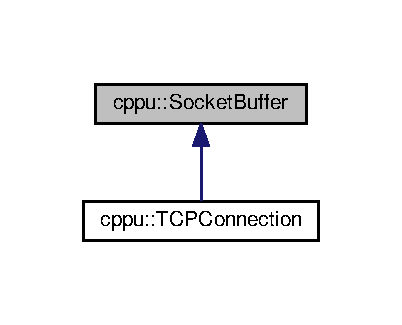
\includegraphics[width=193pt]{classcppu_1_1SocketBuffer__inherit__graph}
\end{center}
\end{figure}


Collaboration diagram for cppu\+:\+:Socket\+Buffer\+:\nopagebreak
\begin{figure}[H]
\begin{center}
\leavevmode
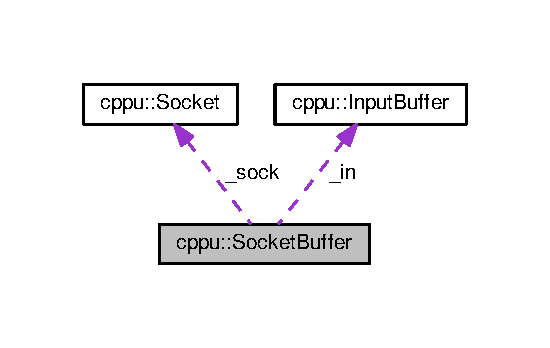
\includegraphics[width=264pt]{classcppu_1_1SocketBuffer__coll__graph}
\end{center}
\end{figure}
\subsection*{Public Member Functions}
\begin{DoxyCompactItemize}
\item 
\hyperlink{classcppu_1_1SocketBuffer_a1d6a8ae90bfcb69e6b3d2b9f97e3dc40}{Socket\+Buffer} (\hyperlink{classcppu_1_1Socket}{Socket} $\ast$\hyperlink{classcppu_1_1SocketBuffer_aab887b32ee999bfdd01c9a491c04bd61}{socket}, size\+\_\+t input\+Buffer\+Size=8192, size\+\_\+t ouput\+Buffer\+Size=8192)\hypertarget{classcppu_1_1SocketBuffer_a1d6a8ae90bfcb69e6b3d2b9f97e3dc40}{}\label{classcppu_1_1SocketBuffer_a1d6a8ae90bfcb69e6b3d2b9f97e3dc40}

\begin{DoxyCompactList}\small\item\em constructor. {\itshape socket} must be a connected T\+C\+P/\+IP \hyperlink{classcppu_1_1Socket}{Socket} (i.\+e. of S\+O\+C\+K\+\_\+\+S\+T\+R\+E\+AM type) that must {\itshape not} be deleted while the \hyperlink{classcppu_1_1SocketBuffer}{Socket\+Buffer} is used. {\itshape input\+Buffer\+Size} and {\itshape ouput\+Buffer\+Size} are the sizes of the buffers that used internally for exchanging the data. \end{DoxyCompactList}\item 
{\bfseries Socket\+Buffer} (\hyperlink{classcppu_1_1Socket}{Socket} \&\hyperlink{classcppu_1_1SocketBuffer_aab887b32ee999bfdd01c9a491c04bd61}{socket}, size\+\_\+t input\+Buffer\+Size=8192, size\+\_\+t ouput\+Buffer\+Size=8192)\hypertarget{classcppu_1_1SocketBuffer_ae8e387747f17f4ff3bfe036ccf11e89b}{}\label{classcppu_1_1SocketBuffer_ae8e387747f17f4ff3bfe036ccf11e89b}

\item 
\hyperlink{classcppu_1_1Socket}{Socket} $\ast$ \hyperlink{classcppu_1_1SocketBuffer_aab887b32ee999bfdd01c9a491c04bd61}{socket} ()\hypertarget{classcppu_1_1SocketBuffer_aab887b32ee999bfdd01c9a491c04bd61}{}\label{classcppu_1_1SocketBuffer_aab887b32ee999bfdd01c9a491c04bd61}

\begin{DoxyCompactList}\small\item\em returns the associated socket. \end{DoxyCompactList}\item 
int \hyperlink{classcppu_1_1SocketBuffer_a77dfe31ad3d5660322d788daf213534e}{input\+Separator} () const \hypertarget{classcppu_1_1SocketBuffer_a77dfe31ad3d5660322d788daf213534e}{}\label{classcppu_1_1SocketBuffer_a77dfe31ad3d5660322d788daf213534e}

\begin{DoxyCompactList}\small\item\em returns the input separator. \end{DoxyCompactList}\item 
int \hyperlink{classcppu_1_1SocketBuffer_a737c72f4ce5ff73a2e7339430b6d1614}{output\+Separator} () const \hypertarget{classcppu_1_1SocketBuffer_a737c72f4ce5ff73a2e7339430b6d1614}{}\label{classcppu_1_1SocketBuffer_a737c72f4ce5ff73a2e7339430b6d1614}

\begin{DoxyCompactList}\small\item\em returns the output separator. \end{DoxyCompactList}\item 
virtual void \hyperlink{classcppu_1_1SocketBuffer_acadf4540c1e3eba67b014753b84b482c}{set\+Input\+Separator} (int separ)
\begin{DoxyCompactList}\small\item\em changes the input separator. This function specifies the character(s) used by \hyperlink{classcppu_1_1SocketBuffer_a222769d3776b9cbd3a727ee1f0e60358}{read\+Line()} to separate successive lines\+: \end{DoxyCompactList}\item 
virtual void \hyperlink{classcppu_1_1SocketBuffer_a0e5e6a9ce3bda28b65c559c8b3c91b0f}{set\+Output\+Separator} (int separ)
\begin{DoxyCompactList}\small\item\em changes the output separator. This function specifies the character(s) used by \hyperlink{classcppu_1_1SocketBuffer_a92ae0351aaee8719d34e8c4618495d59}{write\+Line()} to separate successive lines\+: \end{DoxyCompactList}\item 
virtual ssize\+\_\+t \hyperlink{classcppu_1_1SocketBuffer_a222769d3776b9cbd3a727ee1f0e60358}{read\+Line} (std\+::string \&str)
\begin{DoxyCompactList}\small\item\em Reads a line of text from a connected socket. \hyperlink{classcppu_1_1SocketBuffer_a222769d3776b9cbd3a727ee1f0e60358}{read\+Line()} receives one line of text sent by \hyperlink{classcppu_1_1SocketBuffer_a92ae0351aaee8719d34e8c4618495d59}{write\+Line()} on the other side. The text is stored in {\itshape str}. This method blocks until the complete text line is received. \end{DoxyCompactList}\item 
virtual ssize\+\_\+t \hyperlink{classcppu_1_1SocketBuffer_a92ae0351aaee8719d34e8c4618495d59}{write\+Line} (const std\+::string \&str)
\begin{DoxyCompactList}\small\item\em Sends a line of text to a connected socket. \hyperlink{classcppu_1_1SocketBuffer_a92ae0351aaee8719d34e8c4618495d59}{write\+Line()} sends one line of text that will be received by a single call to \hyperlink{classcppu_1_1SocketBuffer_a222769d3776b9cbd3a727ee1f0e60358}{read\+Line()} on the other side (see note below). \end{DoxyCompactList}\item 
virtual ssize\+\_\+t {\bfseries read} (char $\ast$buffer, size\+\_\+t len)\hypertarget{classcppu_1_1SocketBuffer_a27de273ae2defbf3a5cc308310b9835e}{}\label{classcppu_1_1SocketBuffer_a27de273ae2defbf3a5cc308310b9835e}

\item 
virtual ssize\+\_\+t {\bfseries write} (const char $\ast$str, size\+\_\+t len)\hypertarget{classcppu_1_1SocketBuffer_ab4ed032f329be2f6ecd0cba5fcd0518d}{}\label{classcppu_1_1SocketBuffer_ab4ed032f329be2f6ecd0cba5fcd0518d}

\end{DoxyCompactItemize}
\subsection*{Protected Member Functions}
\begin{DoxyCompactItemize}
\item 
virtual bool {\bfseries retrieve\+Line} (std\+::string \&str, ssize\+\_\+t received)\hypertarget{classcppu_1_1SocketBuffer_ae634cbe12f6688a8d64c4579299e9802}{}\label{classcppu_1_1SocketBuffer_ae634cbe12f6688a8d64c4579299e9802}

\end{DoxyCompactItemize}
\subsection*{Protected Attributes}
\begin{DoxyCompactItemize}
\item 
size\+\_\+t {\bfseries \+\_\+in\+Size}\hypertarget{classcppu_1_1SocketBuffer_af52d0e7a5fb70ad371693c2e7f9f056b}{}\label{classcppu_1_1SocketBuffer_af52d0e7a5fb70ad371693c2e7f9f056b}

\item 
size\+\_\+t {\bfseries \+\_\+out\+Size}\hypertarget{classcppu_1_1SocketBuffer_afa2daeed2c8538030353382f48269896}{}\label{classcppu_1_1SocketBuffer_afa2daeed2c8538030353382f48269896}

\item 
int {\bfseries \+\_\+in\+Sep}\hypertarget{classcppu_1_1SocketBuffer_a5bf8f3a5ef56fc6f15ade71fe55b049d}{}\label{classcppu_1_1SocketBuffer_a5bf8f3a5ef56fc6f15ade71fe55b049d}

\item 
int {\bfseries \+\_\+out\+Sep}\hypertarget{classcppu_1_1SocketBuffer_a59b35cfa717476d18cc2e40c73073354}{}\label{classcppu_1_1SocketBuffer_a59b35cfa717476d18cc2e40c73073354}

\item 
\hyperlink{classcppu_1_1Socket}{Socket} $\ast$ {\bfseries \+\_\+sock}\hypertarget{classcppu_1_1SocketBuffer_af60722acd94826d780bbb2477667d538}{}\label{classcppu_1_1SocketBuffer_af60722acd94826d780bbb2477667d538}

\item 
struct \hyperlink{structcppu_1_1InputBuffer}{Input\+Buffer} $\ast$ {\bfseries \+\_\+in}\hypertarget{classcppu_1_1SocketBuffer_adb5986d6297496a1f92a30b1b3923072}{}\label{classcppu_1_1SocketBuffer_adb5986d6297496a1f92a30b1b3923072}

\end{DoxyCompactItemize}


\subsection{Detailed Description}
Preserves record boundaries when exchanging data between connected T\+C\+P/\+IP sockets. This class ensures that one call to \hyperlink{classcppu_1_1SocketBuffer_a92ae0351aaee8719d34e8c4618495d59}{write\+Line()} corresponds to one and exactly one call to \hyperlink{classcppu_1_1SocketBuffer_a222769d3776b9cbd3a727ee1f0e60358}{read\+Line()} on the other side. This differs from the behavior of \hyperlink{classcppu_1_1Socket_aeac77f859159715e2d63a5a0dc118788}{Socket\+::send()} and \hyperlink{classcppu_1_1Socket_a37c382af52cc02f92c0e19a0c6e0e04f}{Socket\+::receive()} because T\+C\+P/\+IP connected sockets do not preserve record boundaries. \hyperlink{classcppu_1_1SocketBuffer_a92ae0351aaee8719d34e8c4618495d59}{write\+Line()} and \hyperlink{classcppu_1_1SocketBuffer_a222769d3776b9cbd3a727ee1f0e60358}{read\+Line()} solve this problem by automatically adding and searching for a separator between successive lines. 

\begin{DoxySeeAlso}{See also}
\hyperlink{classcppu_1_1SocketBuffer_acadf4540c1e3eba67b014753b84b482c}{set\+Input\+Separator()} and \hyperlink{classcppu_1_1SocketBuffer_a0e5e6a9ce3bda28b65c559c8b3c91b0f}{set\+Output\+Separator()}. 
\end{DoxySeeAlso}


\subsection{Member Function Documentation}
\index{cppu\+::\+Socket\+Buffer@{cppu\+::\+Socket\+Buffer}!read\+Line@{read\+Line}}
\index{read\+Line@{read\+Line}!cppu\+::\+Socket\+Buffer@{cppu\+::\+Socket\+Buffer}}
\subsubsection[{\texorpdfstring{read\+Line(std\+::string \&str)}{readLine(std::string &str)}}]{\setlength{\rightskip}{0pt plus 5cm}ssize\+\_\+t cppu\+::\+Socket\+Buffer\+::read\+Line (
\begin{DoxyParamCaption}
\item[{std\+::string \&}]{str}
\end{DoxyParamCaption}
)\hspace{0.3cm}{\ttfamily [virtual]}}\hypertarget{classcppu_1_1SocketBuffer_a222769d3776b9cbd3a727ee1f0e60358}{}\label{classcppu_1_1SocketBuffer_a222769d3776b9cbd3a727ee1f0e60358}


Reads a line of text from a connected socket. \hyperlink{classcppu_1_1SocketBuffer_a222769d3776b9cbd3a727ee1f0e60358}{read\+Line()} receives one line of text sent by \hyperlink{classcppu_1_1SocketBuffer_a92ae0351aaee8719d34e8c4618495d59}{write\+Line()} on the other side. The text is stored in {\itshape str}. This method blocks until the complete text line is received. 

\hyperlink{classcppu_1_1SocketBuffer_a222769d3776b9cbd3a727ee1f0e60358}{read\+Line()} relies on a separator (by default, ~\newline
, ~\newline
 or ~\newline
, \begin{DoxySeeAlso}{See also}
\hyperlink{classcppu_1_1SocketBuffer_acadf4540c1e3eba67b014753b84b482c}{set\+Input\+Separator()}. This separator is automatically removed (it is not stored in {\itshape str}).
\end{DoxySeeAlso}
\begin{DoxyReturn}{Returns}
the number of bytes that were received or\+:
\begin{DoxyItemize}
\item 0\+: shutdown\+Output() was called on the other side
\item Socket\+::\+Failed (-\/1)\+: a connection error occured
\item Socket\+::\+Invalid\+Socket (-\/2)\+: the socket is invalid. The separator is counted in the value returned by \hyperlink{classcppu_1_1SocketBuffer_a222769d3776b9cbd3a727ee1f0e60358}{read\+Line()}. 
\end{DoxyItemize}
\end{DoxyReturn}
\index{cppu\+::\+Socket\+Buffer@{cppu\+::\+Socket\+Buffer}!set\+Input\+Separator@{set\+Input\+Separator}}
\index{set\+Input\+Separator@{set\+Input\+Separator}!cppu\+::\+Socket\+Buffer@{cppu\+::\+Socket\+Buffer}}
\subsubsection[{\texorpdfstring{set\+Input\+Separator(int separ)}{setInputSeparator(int separ)}}]{\setlength{\rightskip}{0pt plus 5cm}void cppu\+::\+Socket\+Buffer\+::set\+Input\+Separator (
\begin{DoxyParamCaption}
\item[{int}]{separ}
\end{DoxyParamCaption}
)\hspace{0.3cm}{\ttfamily [virtual]}}\hypertarget{classcppu_1_1SocketBuffer_acadf4540c1e3eba67b014753b84b482c}{}\label{classcppu_1_1SocketBuffer_acadf4540c1e3eba67b014753b84b482c}


changes the input separator. This function specifies the character(s) used by \hyperlink{classcppu_1_1SocketBuffer_a222769d3776b9cbd3a727ee1f0e60358}{read\+Line()} to separate successive lines\+: 


\begin{DoxyItemize}
\item if {\itshape separ} $>$= 0, \hyperlink{classcppu_1_1SocketBuffer_a222769d3776b9cbd3a727ee1f0e60358}{read\+Line()} searches for {\itshape separ} to separate lines,
\item if {\itshape separ} $<$ 0, \hyperlink{classcppu_1_1SocketBuffer_a222769d3776b9cbd3a727ee1f0e60358}{read\+Line()} searches for ~\newline
,  or ~\newline
. By default, \hyperlink{classcppu_1_1SocketBuffer_a222769d3776b9cbd3a727ee1f0e60358}{read\+Line()} for ~\newline
,  or ~\newline
. \begin{DoxyNote}{Note}
If the input separator is changed, the output separator must be changed accordingly on the other side of the socket. 
\end{DoxyNote}
\begin{DoxySeeAlso}{See also}
\hyperlink{classcppu_1_1SocketBuffer_a0e5e6a9ce3bda28b65c559c8b3c91b0f}{set\+Output\+Separator()}. 
\end{DoxySeeAlso}

\end{DoxyItemize}\index{cppu\+::\+Socket\+Buffer@{cppu\+::\+Socket\+Buffer}!set\+Output\+Separator@{set\+Output\+Separator}}
\index{set\+Output\+Separator@{set\+Output\+Separator}!cppu\+::\+Socket\+Buffer@{cppu\+::\+Socket\+Buffer}}
\subsubsection[{\texorpdfstring{set\+Output\+Separator(int separ)}{setOutputSeparator(int separ)}}]{\setlength{\rightskip}{0pt plus 5cm}void cppu\+::\+Socket\+Buffer\+::set\+Output\+Separator (
\begin{DoxyParamCaption}
\item[{int}]{separ}
\end{DoxyParamCaption}
)\hspace{0.3cm}{\ttfamily [virtual]}}\hypertarget{classcppu_1_1SocketBuffer_a0e5e6a9ce3bda28b65c559c8b3c91b0f}{}\label{classcppu_1_1SocketBuffer_a0e5e6a9ce3bda28b65c559c8b3c91b0f}


changes the output separator. This function specifies the character(s) used by \hyperlink{classcppu_1_1SocketBuffer_a92ae0351aaee8719d34e8c4618495d59}{write\+Line()} to separate successive lines\+: 


\begin{DoxyItemize}
\item if {\itshape separ} $>$= 0, \hyperlink{classcppu_1_1SocketBuffer_a92ae0351aaee8719d34e8c4618495d59}{write\+Line()} inserts {\itshape separ} between successive lines,
\item if {\itshape separ} $<$ 0, \hyperlink{classcppu_1_1SocketBuffer_a92ae0351aaee8719d34e8c4618495d59}{write\+Line()} inserts ~\newline
 between successive lines. By default, \hyperlink{classcppu_1_1SocketBuffer_a92ae0351aaee8719d34e8c4618495d59}{write\+Line()} inserts ~\newline
. \begin{DoxyNote}{Note}
If the output separator is changed, the input separator must be changed accordingly on the other side of the socket. 
\end{DoxyNote}
\begin{DoxySeeAlso}{See also}
\hyperlink{classcppu_1_1SocketBuffer_acadf4540c1e3eba67b014753b84b482c}{set\+Input\+Separator()}. 
\end{DoxySeeAlso}

\end{DoxyItemize}\index{cppu\+::\+Socket\+Buffer@{cppu\+::\+Socket\+Buffer}!write\+Line@{write\+Line}}
\index{write\+Line@{write\+Line}!cppu\+::\+Socket\+Buffer@{cppu\+::\+Socket\+Buffer}}
\subsubsection[{\texorpdfstring{write\+Line(const std\+::string \&str)}{writeLine(const std::string &str)}}]{\setlength{\rightskip}{0pt plus 5cm}ssize\+\_\+t cppu\+::\+Socket\+Buffer\+::write\+Line (
\begin{DoxyParamCaption}
\item[{const std\+::string \&}]{str}
\end{DoxyParamCaption}
)\hspace{0.3cm}{\ttfamily [virtual]}}\hypertarget{classcppu_1_1SocketBuffer_a92ae0351aaee8719d34e8c4618495d59}{}\label{classcppu_1_1SocketBuffer_a92ae0351aaee8719d34e8c4618495d59}


Sends a line of text to a connected socket. \hyperlink{classcppu_1_1SocketBuffer_a92ae0351aaee8719d34e8c4618495d59}{write\+Line()} sends one line of text that will be received by a single call to \hyperlink{classcppu_1_1SocketBuffer_a222769d3776b9cbd3a727ee1f0e60358}{read\+Line()} on the other side (see note below). 

\hyperlink{classcppu_1_1SocketBuffer_a92ae0351aaee8719d34e8c4618495d59}{write\+Line()} relies on a separator (~\newline
 by default, \begin{DoxySeeAlso}{See also}
\hyperlink{classcppu_1_1SocketBuffer_a0e5e6a9ce3bda28b65c559c8b3c91b0f}{set\+Output\+Separator()}) that is automatically inserted between successive lines ().
\end{DoxySeeAlso}
\begin{DoxyReturn}{Returns}
the number of bytes that were sent or\+:
\begin{DoxyItemize}
\item 0\+: shutdown\+Input() was called on the other side
\item Socket\+::\+Failed (-\/1)\+: a connection error occured
\item Socket\+::\+Invalid\+Socket (-\/2)\+: the socket is invalid. The separator is counted in the value returned by \hyperlink{classcppu_1_1SocketBuffer_a92ae0351aaee8719d34e8c4618495d59}{write\+Line()}.
\end{DoxyItemize}
\end{DoxyReturn}
\begin{DoxyNote}{Note}
if {\itshape str} constains occurences of the separator, \hyperlink{classcppu_1_1SocketBuffer_a222769d3776b9cbd3a727ee1f0e60358}{read\+Line()} will be called several times on the other side. 
\end{DoxyNote}


The documentation for this class was generated from the following files\+:\begin{DoxyCompactItemize}
\item 
cppsocket.\+h\item 
cppsocket.\+cpp\end{DoxyCompactItemize}

\hypertarget{classcppu_1_1TCPConnection}{}\section{cppu\+:\+:T\+C\+P\+Connection Class Reference}
\label{classcppu_1_1TCPConnection}\index{cppu\+::\+T\+C\+P\+Connection@{cppu\+::\+T\+C\+P\+Connection}}


Connection with a given client. Each \hyperlink{classcppu_1_1TCPConnection}{T\+C\+P\+Connection} uses a different thread.  




{\ttfamily \#include $<$tcpserver.\+h$>$}



Inheritance diagram for cppu\+:\+:T\+C\+P\+Connection\+:\nopagebreak
\begin{figure}[H]
\begin{center}
\leavevmode
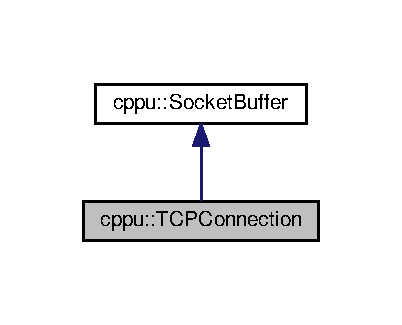
\includegraphics[width=193pt]{classcppu_1_1TCPConnection__inherit__graph}
\end{center}
\end{figure}


Collaboration diagram for cppu\+:\+:T\+C\+P\+Connection\+:\nopagebreak
\begin{figure}[H]
\begin{center}
\leavevmode
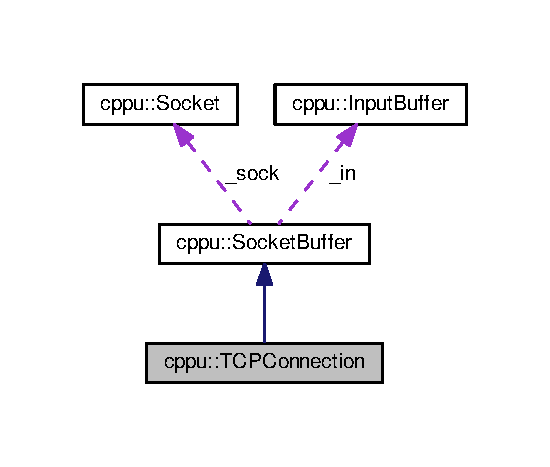
\includegraphics[width=264pt]{classcppu_1_1TCPConnection__coll__graph}
\end{center}
\end{figure}
\subsection*{Public Member Functions}
\begin{DoxyCompactItemize}
\item 
\hyperlink{classcppu_1_1TCPServer}{T\+C\+P\+Server} \& {\bfseries server} ()\hypertarget{classcppu_1_1TCPConnection_a4186946c7c22e3c2cebe3a97aa78f5f7}{}\label{classcppu_1_1TCPConnection_a4186946c7c22e3c2cebe3a97aa78f5f7}

\item 
pthread\+\_\+t {\bfseries thread} ()\hypertarget{classcppu_1_1TCPConnection_a4663875b80fced790502880c72e6e672}{}\label{classcppu_1_1TCPConnection_a4663875b80fced790502880c72e6e672}

\end{DoxyCompactItemize}
\subsection*{Friends}
\begin{DoxyCompactItemize}
\item 
class {\bfseries T\+C\+P\+Server}\hypertarget{classcppu_1_1TCPConnection_ae4cfdb1814d91a8d28dadb49adda68f0}{}\label{classcppu_1_1TCPConnection_ae4cfdb1814d91a8d28dadb49adda68f0}

\end{DoxyCompactItemize}
\subsection*{Additional Inherited Members}


\subsection{Detailed Description}
Connection with a given client. Each \hyperlink{classcppu_1_1TCPConnection}{T\+C\+P\+Connection} uses a different thread. 

The documentation for this class was generated from the following files\+:\begin{DoxyCompactItemize}
\item 
tcpserver.\+h\item 
tcpserver.\+cpp\end{DoxyCompactItemize}

\hypertarget{classcppu_1_1TCPLock}{}\section{cppu\+:\+:T\+C\+P\+Lock Class Reference}
\label{classcppu_1_1TCPLock}\index{cppu\+::\+T\+C\+P\+Lock@{cppu\+::\+T\+C\+P\+Lock}}


Locks the server in read mode or in write mode. Must be created {\itshape in the stack} by the callback method.  




{\ttfamily \#include $<$tcpserver.\+h$>$}

\subsection*{Public Member Functions}
\begin{DoxyCompactItemize}
\item 
\hyperlink{classcppu_1_1TCPLock_ad9ff8205f334918a69746ef90f731877}{T\+C\+P\+Lock} (\hyperlink{classcppu_1_1TCPConnection}{T\+C\+P\+Connection} \&cnx, bool write\+Mode=false)
\begin{DoxyCompactList}\small\item\em locks the server in {\itshape write} or {\itshape read} mode. In order to avoid concurrency problems between threads, the callback method ( \end{DoxyCompactList}\end{DoxyCompactItemize}


\subsection{Detailed Description}
Locks the server in read mode or in write mode. Must be created {\itshape in the stack} by the callback method. 

\subsection{Constructor \& Destructor Documentation}
\index{cppu\+::\+T\+C\+P\+Lock@{cppu\+::\+T\+C\+P\+Lock}!T\+C\+P\+Lock@{T\+C\+P\+Lock}}
\index{T\+C\+P\+Lock@{T\+C\+P\+Lock}!cppu\+::\+T\+C\+P\+Lock@{cppu\+::\+T\+C\+P\+Lock}}
\subsubsection[{\texorpdfstring{T\+C\+P\+Lock(\+T\+C\+P\+Connection \&cnx, bool write\+Mode=false)}{TCPLock(TCPConnection &cnx, bool writeMode=false)}}]{\setlength{\rightskip}{0pt plus 5cm}cppu\+::\+T\+C\+P\+Lock\+::\+T\+C\+P\+Lock (
\begin{DoxyParamCaption}
\item[{{\bf T\+C\+P\+Connection} \&}]{cnx, }
\item[{bool}]{write\+Mode = {\ttfamily false}}
\end{DoxyParamCaption}
)}\hypertarget{classcppu_1_1TCPLock_ad9ff8205f334918a69746ef90f731877}{}\label{classcppu_1_1TCPLock_ad9ff8205f334918a69746ef90f731877}


locks the server in {\itshape write} or {\itshape read} mode. In order to avoid concurrency problems between threads, the callback method ( 

\begin{DoxySeeAlso}{See also}
set\+Callback()) can create a \hyperlink{classcppu_1_1TCPLock}{T\+C\+P\+Lock} object {\itshape in the stack} before performing a computation.
\end{DoxySeeAlso}
{\itshape write\+Mode} must be true if the callback changes data and false (the default) otherwise. A write\+Mode lock blocks all other locks (and the corresponding threads) until the callback method returns. 

The documentation for this class was generated from the following files\+:\begin{DoxyCompactItemize}
\item 
tcpserver.\+h\item 
tcpserver.\+cpp\end{DoxyCompactItemize}

\hypertarget{classcppu_1_1TCPServer}{}\section{cppu\+:\+:T\+C\+P\+Server Class Reference}
\label{classcppu_1_1TCPServer}\index{cppu\+::\+T\+C\+P\+Server@{cppu\+::\+T\+C\+P\+Server}}


T\+C\+P/\+IP I\+Pv4 server. The server supports T\+C\+P/\+IP A\+F\+\_\+\+I\+N\+ET connections (following the I\+Pv4 Internet protocol) with multiple clients. One thread is used per client.  




{\ttfamily \#include $<$tcpserver.\+h$>$}



Collaboration diagram for cppu\+:\+:T\+C\+P\+Server\+:\nopagebreak
\begin{figure}[H]
\begin{center}
\leavevmode
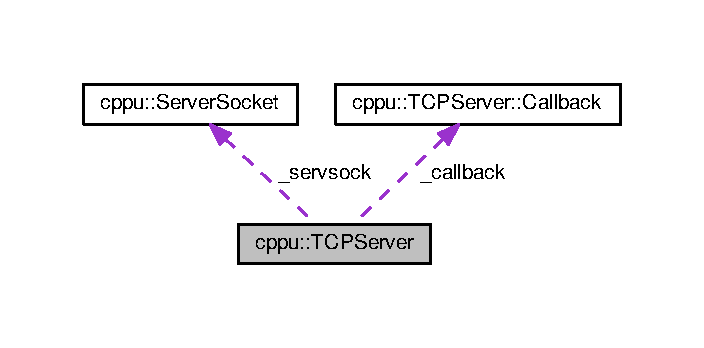
\includegraphics[width=338pt]{classcppu_1_1TCPServer__coll__graph}
\end{center}
\end{figure}
\subsection*{Classes}
\begin{DoxyCompactItemize}
\item 
struct \hyperlink{structcppu_1_1TCPServer_1_1Callback}{Callback}
\begin{DoxyCompactList}\small\item\em \hyperlink{structcppu_1_1TCPServer_1_1Callback}{Callback} interface. \end{DoxyCompactList}\item 
struct \hyperlink{structcppu_1_1TCPServer_1_1CallbackMethod}{Callback\+Method}
\end{DoxyCompactItemize}
\subsection*{Public Member Functions}
\begin{DoxyCompactItemize}
\item 
\hyperlink{classcppu_1_1TCPServer_a48074f8409f580f6cf7b0be80200f9f3}{T\+C\+P\+Server} ()\hypertarget{classcppu_1_1TCPServer_a48074f8409f580f6cf7b0be80200f9f3}{}\label{classcppu_1_1TCPServer_a48074f8409f580f6cf7b0be80200f9f3}

\begin{DoxyCompactList}\small\item\em constructor\+: initializes the \hyperlink{classcppu_1_1TCPServer}{T\+C\+P\+Server}. \end{DoxyCompactList}\item 
virtual \hyperlink{classcppu_1_1TCPServer_ababd20111e0cf4e14396433e56ca086e}{$\sim$\+T\+C\+P\+Server} ()\hypertarget{classcppu_1_1TCPServer_ababd20111e0cf4e14396433e56ca086e}{}\label{classcppu_1_1TCPServer_ababd20111e0cf4e14396433e56ca086e}

\begin{DoxyCompactList}\small\item\em destructor\+: cleans up the \hyperlink{classcppu_1_1TCPServer}{T\+C\+P\+Server}. \end{DoxyCompactList}\item 
virtual int \hyperlink{classcppu_1_1TCPServer_a98e00d62745812b17bdee9f07f2070c4}{run} (int port)
\begin{DoxyCompactList}\small\item\em starts the \hyperlink{classcppu_1_1TCPServer}{T\+C\+P\+Server}. \hyperlink{classcppu_1_1TCPServer_a98e00d62745812b17bdee9f07f2070c4}{run()} binds an internal \hyperlink{classcppu_1_1ServerSocket}{Server\+Socket} to {\itshape port} then starts an infinite loop that processes connection requests from clients. \end{DoxyCompactList}\item 
{\footnotesize template$<$class T $>$ }\\void \hyperlink{classcppu_1_1TCPServer_a7d4fdb93439015934004755fde72945b}{set\+Callback} (T \&object, bool(T\+::$\ast$method)(\hyperlink{classcppu_1_1TCPConnection}{T\+C\+P\+Connection} \&cnx, const std\+::string \&request, std\+::string \&response))
\begin{DoxyCompactList}\small\item\em changes the callback method of the \hyperlink{classcppu_1_1TCPServer}{T\+C\+P\+Server}. This callback is called each time the \hyperlink{classcppu_1_1TCPServer}{T\+C\+P\+Server} receives a request from a client. It can be any method of {\itshape object} with the following parameters\+: \end{DoxyCompactList}\item 
void \hyperlink{classcppu_1_1TCPServer_a94d3d97b03d5e3e48609e405d8dd7897}{set\+Callback} (\hyperlink{structcppu_1_1TCPServer_1_1Callback}{Callback} \&callback)
\begin{DoxyCompactList}\small\item\em changes the callback object of the \hyperlink{classcppu_1_1TCPServer}{T\+C\+P\+Server}. \end{DoxyCompactList}\item 
\hyperlink{classcppu_1_1ServerSocket}{Server\+Socket} \& \hyperlink{classcppu_1_1TCPServer_a6428b63a4440045050dba4f33bb454bf}{server\+Socket} ()\hypertarget{classcppu_1_1TCPServer_a6428b63a4440045050dba4f33bb454bf}{}\label{classcppu_1_1TCPServer_a6428b63a4440045050dba4f33bb454bf}

\begin{DoxyCompactList}\small\item\em returns the internal \hyperlink{classcppu_1_1ServerSocket}{Server\+Socket}. \end{DoxyCompactList}\item 
virtual void \hyperlink{classcppu_1_1TCPServer_afc47ca4476d9c75d5ea88f73e2acd6d5}{error} (const std\+::string \&msg, const \hyperlink{classcppu_1_1TCPConnection}{T\+C\+P\+Connection} $\ast$=nullptr)\hypertarget{classcppu_1_1TCPServer_afc47ca4476d9c75d5ea88f73e2acd6d5}{}\label{classcppu_1_1TCPServer_afc47ca4476d9c75d5ea88f73e2acd6d5}

\begin{DoxyCompactList}\small\item\em prints warning and error messages on the terminal. \end{DoxyCompactList}\end{DoxyCompactItemize}
\subsection*{Protected Member Functions}
\begin{DoxyCompactItemize}
\item 
virtual \hyperlink{classcppu_1_1TCPConnection}{T\+C\+P\+Connection} $\ast$ \hyperlink{classcppu_1_1TCPServer_abe314b95a31c88b479c81ec9bf123c65}{create\+Cnx} (\hyperlink{classcppu_1_1Socket}{Socket} $\ast$)\hypertarget{classcppu_1_1TCPServer_abe314b95a31c88b479c81ec9bf123c65}{}\label{classcppu_1_1TCPServer_abe314b95a31c88b479c81ec9bf123c65}

\begin{DoxyCompactList}\small\item\em creates a new connection that starts a new thread for listening this socket. \end{DoxyCompactList}\end{DoxyCompactItemize}
\subsection*{Protected Attributes}
\begin{DoxyCompactItemize}
\item 
\hyperlink{classcppu_1_1ServerSocket}{Server\+Socket} {\bfseries \+\_\+servsock}\hypertarget{classcppu_1_1TCPServer_a8e4422abf23dc5bd195d05a3e9eee167}{}\label{classcppu_1_1TCPServer_a8e4422abf23dc5bd195d05a3e9eee167}

\item 
std\+::shared\+\_\+ptr$<$ \hyperlink{structcppu_1_1TCPServer_1_1Callback}{Callback} $>$ {\bfseries \+\_\+callback\+Ptr}\hypertarget{classcppu_1_1TCPServer_abe36d427d7b047cdd342e282611c841e}{}\label{classcppu_1_1TCPServer_abe36d427d7b047cdd342e282611c841e}

\item 
\hyperlink{structcppu_1_1TCPServer_1_1Callback}{Callback} $\ast$ {\bfseries \+\_\+callback}\hypertarget{classcppu_1_1TCPServer_a68940bd70ac6941ca49d1e51b631f5e9}{}\label{classcppu_1_1TCPServer_a68940bd70ac6941ca49d1e51b631f5e9}

\item 
pthread\+\_\+rwlock\+\_\+t {\bfseries \+\_\+threadlock}\hypertarget{classcppu_1_1TCPServer_aea2dbb4b5762044217096e52cd559b97}{}\label{classcppu_1_1TCPServer_aea2dbb4b5762044217096e52cd559b97}

\end{DoxyCompactItemize}
\subsection*{Friends}
\begin{DoxyCompactItemize}
\item 
class {\bfseries T\+C\+P\+Lock}\hypertarget{classcppu_1_1TCPServer_a94abdeb80587f39a869fde6f24522a78}{}\label{classcppu_1_1TCPServer_a94abdeb80587f39a869fde6f24522a78}

\item 
class {\bfseries T\+C\+P\+Connection}\hypertarget{classcppu_1_1TCPServer_a9d1c27bdfcdd48c5f07a5d0dce43b346}{}\label{classcppu_1_1TCPServer_a9d1c27bdfcdd48c5f07a5d0dce43b346}

\end{DoxyCompactItemize}


\subsection{Detailed Description}
T\+C\+P/\+IP I\+Pv4 server. The server supports T\+C\+P/\+IP A\+F\+\_\+\+I\+N\+ET connections (following the I\+Pv4 Internet protocol) with multiple clients. One thread is used per client. 

Call \hyperlink{classcppu_1_1TCPServer_a7d4fdb93439015934004755fde72945b}{set\+Callback()} to specify the callback method that will be invoked each time a request is sent by a client then \hyperlink{classcppu_1_1TCPServer_a98e00d62745812b17bdee9f07f2070c4}{run()} to start the server.

Requests can be processed concurrently thanks to threads. To avoid concurrency problems the callback can perform a read or write lock (\begin{DoxySeeAlso}{See also}
\hyperlink{classcppu_1_1TCPLock}{T\+C\+P\+Lock}). 
\end{DoxySeeAlso}


\subsection{Member Function Documentation}
\index{cppu\+::\+T\+C\+P\+Server@{cppu\+::\+T\+C\+P\+Server}!run@{run}}
\index{run@{run}!cppu\+::\+T\+C\+P\+Server@{cppu\+::\+T\+C\+P\+Server}}
\subsubsection[{\texorpdfstring{run(int port)}{run(int port)}}]{\setlength{\rightskip}{0pt plus 5cm}int cppu\+::\+T\+C\+P\+Server\+::run (
\begin{DoxyParamCaption}
\item[{int}]{port}
\end{DoxyParamCaption}
)\hspace{0.3cm}{\ttfamily [virtual]}}\hypertarget{classcppu_1_1TCPServer_a98e00d62745812b17bdee9f07f2070c4}{}\label{classcppu_1_1TCPServer_a98e00d62745812b17bdee9f07f2070c4}


starts the \hyperlink{classcppu_1_1TCPServer}{T\+C\+P\+Server}. \hyperlink{classcppu_1_1TCPServer_a98e00d62745812b17bdee9f07f2070c4}{run()} binds an internal \hyperlink{classcppu_1_1ServerSocket}{Server\+Socket} to {\itshape port} then starts an infinite loop that processes connection requests from clients. 

For each successful connection request, a \hyperlink{classcppu_1_1TCPConnection}{T\+C\+P\+Connection} object is created. This object starts a thread that processes incoming requests from its client. A callback method (\begin{DoxySeeAlso}{See also}
\hyperlink{classcppu_1_1TCPServer_a7d4fdb93439015934004755fde72945b}{set\+Callback()}) is invoked for each request.
\end{DoxySeeAlso}
\begin{DoxyReturn}{Returns}
0 on normal termination or a negative value if the \hyperlink{classcppu_1_1ServerSocket}{Server\+Socket} could not be bound (value is then one of \hyperlink{classcppu_1_1Socket_a49ea5cb079bd7ae97ecf7eb30c9d9e5f}{Socket\+::\+Errors}). 
\end{DoxyReturn}
\index{cppu\+::\+T\+C\+P\+Server@{cppu\+::\+T\+C\+P\+Server}!set\+Callback@{set\+Callback}}
\index{set\+Callback@{set\+Callback}!cppu\+::\+T\+C\+P\+Server@{cppu\+::\+T\+C\+P\+Server}}
\subsubsection[{\texorpdfstring{set\+Callback(\+T \&object, bool(\+T\+::$\ast$method)(\+T\+C\+P\+Connection \&cnx, const std\+::string \&request, std\+::string \&response))}{setCallback(T &object, bool(T::*method)(TCPConnection &cnx, const std::string &request, std::string &response))}}]{\setlength{\rightskip}{0pt plus 5cm}template$<$class T $>$ void cppu\+::\+T\+C\+P\+Server\+::set\+Callback (
\begin{DoxyParamCaption}
\item[{T \&}]{object, }
\item[{bool(T\+::$\ast$)({\bf T\+C\+P\+Connection} \&cnx, const std\+::string \&request, std\+::string \&response)}]{method}
\end{DoxyParamCaption}
)\hspace{0.3cm}{\ttfamily [inline]}}\hypertarget{classcppu_1_1TCPServer_a7d4fdb93439015934004755fde72945b}{}\label{classcppu_1_1TCPServer_a7d4fdb93439015934004755fde72945b}


changes the callback method of the \hyperlink{classcppu_1_1TCPServer}{T\+C\+P\+Server}. This callback is called each time the \hyperlink{classcppu_1_1TCPServer}{T\+C\+P\+Server} receives a request from a client. It can be any method of {\itshape object} with the following parameters\+: 


\begin{DoxyItemize}
\item {\itshape cnx} is the connection with the client sending the request
\item {\itshape request} contains the data sent by the client
\item {\itshape response} will be sent to the client as a response The connection is closed if the callback returns false.
\end{DoxyItemize}

To avoid concurrency problems, the callback should perform a read or write lock (\begin{DoxySeeAlso}{See also}
\hyperlink{classcppu_1_1TCPLock}{T\+C\+P\+Lock}) before performing a computation. 
\end{DoxySeeAlso}
\index{cppu\+::\+T\+C\+P\+Server@{cppu\+::\+T\+C\+P\+Server}!set\+Callback@{set\+Callback}}
\index{set\+Callback@{set\+Callback}!cppu\+::\+T\+C\+P\+Server@{cppu\+::\+T\+C\+P\+Server}}
\subsubsection[{\texorpdfstring{set\+Callback(\+Callback \&callback)}{setCallback(Callback &callback)}}]{\setlength{\rightskip}{0pt plus 5cm}void cppu\+::\+T\+C\+P\+Server\+::set\+Callback (
\begin{DoxyParamCaption}
\item[{{\bf Callback} \&}]{callback}
\end{DoxyParamCaption}
)\hspace{0.3cm}{\ttfamily [inline]}}\hypertarget{classcppu_1_1TCPServer_a94d3d97b03d5e3e48609e405d8dd7897}{}\label{classcppu_1_1TCPServer_a94d3d97b03d5e3e48609e405d8dd7897}


changes the callback object of the \hyperlink{classcppu_1_1TCPServer}{T\+C\+P\+Server}. 

\begin{DoxySeeAlso}{See also}
set\+Callback(object, method). 
\end{DoxySeeAlso}


The documentation for this class was generated from the following files\+:\begin{DoxyCompactItemize}
\item 
tcpserver.\+h\item 
tcpserver.\+cpp\end{DoxyCompactItemize}

\hypertarget{classVideo}{}\section{Video Class Reference}
\label{classVideo}\index{Video@{Video}}


{\ttfamily \#include $<$video.\+h$>$}



Inheritance diagram for Video\+:\nopagebreak
\begin{figure}[H]
\begin{center}
\leavevmode
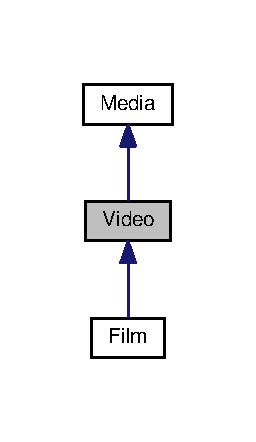
\includegraphics[width=123pt]{classVideo__inherit__graph}
\end{center}
\end{figure}


Collaboration diagram for Video\+:\nopagebreak
\begin{figure}[H]
\begin{center}
\leavevmode
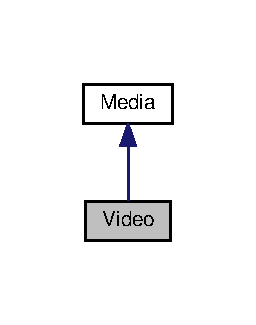
\includegraphics[width=123pt]{classVideo__coll__graph}
\end{center}
\end{figure}
\subsection*{Public Member Functions}
\begin{DoxyCompactItemize}
\item 
virtual \hyperlink{classVideo_aebf7e2a8fa2bbd79335b1cf35925d190}{$\sim$\+Video} ()
\item 
void \hyperlink{classVideo_a28f92e1016a8757ba93211b10f89cdef}{set\+Length} (const int length)
\item 
void \hyperlink{classVideo_acb8fdb5186d3b35672b9218375cf4f0b}{play} () const 
\item 
string \hyperlink{classVideo_ad947c70ddc192dcb8e511fda6a616a4f}{to\+String} () const 
\item 
string \hyperlink{classVideo_a9360aa8a32752c7c732d993f2cf85144}{serialize} () const 
\end{DoxyCompactItemize}
\subsection*{Protected Member Functions}
\begin{DoxyCompactItemize}
\item 
\hyperlink{classVideo_ab67336c2c5b6227a9635bc7dcd6af543}{Video} ()
\item 
\hyperlink{classVideo_a3d83124ab150067cbf5c44f7b54d8a28}{Video} (const string name, const string path\+Name)
\item 
\hyperlink{classVideo_ae46d2c3304be8339b4d4fa73d8e692cb}{Video} (const string serialized)
\end{DoxyCompactItemize}
\subsection*{Protected Attributes}
\begin{DoxyCompactItemize}
\item 
unsigned int \hyperlink{classVideo_a05916bdf80008168a92cee6ebd8eaf25}{v\+\_\+length}
\end{DoxyCompactItemize}


\subsection{Detailed Description}
Represents a video object. 

\subsection{Constructor \& Destructor Documentation}
\index{Video@{Video}!Video@{Video}}
\index{Video@{Video}!Video@{Video}}
\subsubsection[{\texorpdfstring{Video()}{Video()}}]{\setlength{\rightskip}{0pt plus 5cm}Video\+::\+Video (
\begin{DoxyParamCaption}
{}
\end{DoxyParamCaption}
)\hspace{0.3cm}{\ttfamily [protected]}}\hypertarget{classVideo_ab67336c2c5b6227a9635bc7dcd6af543}{}\label{classVideo_ab67336c2c5b6227a9635bc7dcd6af543}
Default constructor \index{Video@{Video}!Video@{Video}}
\index{Video@{Video}!Video@{Video}}
\subsubsection[{\texorpdfstring{Video(const string name, const string path\+Name)}{Video(const string name, const string pathName)}}]{\setlength{\rightskip}{0pt plus 5cm}Video\+::\+Video (
\begin{DoxyParamCaption}
\item[{const string}]{name, }
\item[{const string}]{path\+Name}
\end{DoxyParamCaption}
)\hspace{0.3cm}{\ttfamily [protected]}}\hypertarget{classVideo_a3d83124ab150067cbf5c44f7b54d8a28}{}\label{classVideo_a3d83124ab150067cbf5c44f7b54d8a28}
Creates a new video with a name and a path to the file 
\begin{DoxyParams}{Parameters}
{\em name} & The name of the movie \\
\hline
{\em path\+Name} & the path to the file (relative or absolute) \\
\hline
\end{DoxyParams}
\index{Video@{Video}!Video@{Video}}
\index{Video@{Video}!Video@{Video}}
\subsubsection[{\texorpdfstring{Video(const string serialized)}{Video(const string serialized)}}]{\setlength{\rightskip}{0pt plus 5cm}Video\+::\+Video (
\begin{DoxyParamCaption}
\item[{const string}]{serial}
\end{DoxyParamCaption}
)\hspace{0.3cm}{\ttfamily [protected]}}\hypertarget{classVideo_ae46d2c3304be8339b4d4fa73d8e692cb}{}\label{classVideo_ae46d2c3304be8339b4d4fa73d8e692cb}
Creates a new video with a serialized representation of the movie 
\begin{DoxyParams}{Parameters}
{\em serialized} & a valid serialized representation of the movie, format\+: \char`\"{}\+Video,\mbox{[}name\mbox{]},\mbox{[}path\mbox{]},\mbox{[}length\mbox{]}\char`\"{} e.\+g.\+: \char`\"{}\+Video,dog,$\sim$/\+Videos/dog.\+mkv,345\char`\"{}\\
\hline
\end{DoxyParams}
e.\+g. \char`\"{}\+Video,dog,$\sim$/\+Videos/dog.\+mkv,345\char`\"{} \index{Video@{Video}!````~Video@{$\sim$\+Video}}
\index{````~Video@{$\sim$\+Video}!Video@{Video}}
\subsubsection[{\texorpdfstring{$\sim$\+Video()}{~Video()}}]{\setlength{\rightskip}{0pt plus 5cm}Video\+::$\sim$\+Video (
\begin{DoxyParamCaption}
{}
\end{DoxyParamCaption}
)\hspace{0.3cm}{\ttfamily [virtual]}}\hypertarget{classVideo_aebf7e2a8fa2bbd79335b1cf35925d190}{}\label{classVideo_aebf7e2a8fa2bbd79335b1cf35925d190}
Destroys the object and its components 

\subsection{Member Function Documentation}
\index{Video@{Video}!play@{play}}
\index{play@{play}!Video@{Video}}
\subsubsection[{\texorpdfstring{play() const }{play() const }}]{\setlength{\rightskip}{0pt plus 5cm}void Video\+::play (
\begin{DoxyParamCaption}
{}
\end{DoxyParamCaption}
) const\hspace{0.3cm}{\ttfamily [virtual]}}\hypertarget{classVideo_acb8fdb5186d3b35672b9218375cf4f0b}{}\label{classVideo_acb8fdb5186d3b35672b9218375cf4f0b}
Starts playing the movie. 

Implements \hyperlink{classMedia_aabbaa8413a9eeaccc649f9c3068ddbc6}{Media}.

\index{Video@{Video}!serialize@{serialize}}
\index{serialize@{serialize}!Video@{Video}}
\subsubsection[{\texorpdfstring{serialize() const }{serialize() const }}]{\setlength{\rightskip}{0pt plus 5cm}string Video\+::serialize (
\begin{DoxyParamCaption}
{}
\end{DoxyParamCaption}
) const\hspace{0.3cm}{\ttfamily [virtual]}}\hypertarget{classVideo_a9360aa8a32752c7c732d993f2cf85144}{}\label{classVideo_a9360aa8a32752c7c732d993f2cf85144}
Serializes the object. \begin{DoxyReturn}{Returns}
a string representing the object.
\end{DoxyReturn}
Format\+: \char`\"{}\+Video,\mbox{[}name\mbox{]},\mbox{[}path\mbox{]},\mbox{[}length\mbox{]}\char`\"{}

e.\+g.\+: \char`\"{}\+Video,dog,$\sim$/\+Videos/dog.\+mkv,345\char`\"{} 

Implements \hyperlink{classMedia_ae588d20c062218e43b084da08f2dc5c6}{Media}.

\index{Video@{Video}!set\+Length@{set\+Length}}
\index{set\+Length@{set\+Length}!Video@{Video}}
\subsubsection[{\texorpdfstring{set\+Length(const int length)}{setLength(const int length)}}]{\setlength{\rightskip}{0pt plus 5cm}void Video\+::set\+Length (
\begin{DoxyParamCaption}
\item[{const int}]{length}
\end{DoxyParamCaption}
)}\hypertarget{classVideo_a28f92e1016a8757ba93211b10f89cdef}{}\label{classVideo_a28f92e1016a8757ba93211b10f89cdef}
Set the length of the movie 
\begin{DoxyParams}{Parameters}
{\em length} & The duration of the movie in seconds. \\
\hline
\end{DoxyParams}
\index{Video@{Video}!to\+String@{to\+String}}
\index{to\+String@{to\+String}!Video@{Video}}
\subsubsection[{\texorpdfstring{to\+String() const }{toString() const }}]{\setlength{\rightskip}{0pt plus 5cm}string Video\+::to\+String (
\begin{DoxyParamCaption}
{}
\end{DoxyParamCaption}
) const\hspace{0.3cm}{\ttfamily [virtual]}}\hypertarget{classVideo_ad947c70ddc192dcb8e511fda6a616a4f}{}\label{classVideo_ad947c70ddc192dcb8e511fda6a616a4f}
Prints a representation of the movie in the standard output. 

Implements \hyperlink{classMedia_a95c1c019e23c2e365af1e5093d5232ac}{Media}.



\subsection{Member Data Documentation}
\index{Video@{Video}!v\+\_\+length@{v\+\_\+length}}
\index{v\+\_\+length@{v\+\_\+length}!Video@{Video}}
\subsubsection[{\texorpdfstring{v\+\_\+length}{v_length}}]{\setlength{\rightskip}{0pt plus 5cm}unsigned int Video\+::v\+\_\+length\hspace{0.3cm}{\ttfamily [protected]}}\hypertarget{classVideo_a05916bdf80008168a92cee6ebd8eaf25}{}\label{classVideo_a05916bdf80008168a92cee6ebd8eaf25}
Length of the movie in seconds 

The documentation for this class was generated from the following files\+:\begin{DoxyCompactItemize}
\item 
video.\+h\item 
video.\+cpp\end{DoxyCompactItemize}

%--- End generated contents ---

% Index
\backmatter
\newpage
\phantomsection
\clearemptydoublepage
\addcontentsline{toc}{chapter}{Index}
\printindex

\end{document}
